\documentclass[oneside,openany]{abntex2-ufes}

% Codificação, fonte e qualidade tipográfica
\usepackage[utf8]{inputenc}
\usepackage[T1]{fontenc}
\usepackage{lmodern}
\usepackage{cmap}
\usepackage{microtype}
\usepackage{indentfirst}
\setlength{\emergencystretch}{2em}
\clubpenalty=10000
\widowpenalty=10000
\displaywidowpenalty=10000

% Figuras, tabelas, equações e algoritmos
\usepackage{graphicx}
\usepackage{epstopdf}
\DeclareGraphicsExtensions{.pdf,.jpeg,.eps,.png}
\usepackage{float}
\usepackage{placeins}
\usepackage{tabularx}
\usepackage{longtable}
\usepackage{booktabs}
\usepackage{multirow}
\usepackage{array}
\usepackage{amsfonts,amssymb,amsmath}

% Recursos textuais e elementos pré/pós-textuais
\usepackage[normalem]{ulem}
\usepackage{verbatim}
\usepackage{url}
\usepackage{lastpage}

% Citações e links
\usepackage[
    alf,
    abnt-emphasize=bf,
    recuo=0cm,
    abnt-etal-cite=3,
    abnt-etal-list=0,
    abnt-doi=doi
]{abntex2cite}
\bibliographystyle{abntex2-alf}
\usepackage{hyperref}

% A ABNT NBR 10520:2023 deixou de grafar em caixa alta o autor das
% citações entre parênteses. O abntex2cite distribuído atualmente ainda
% implementa a regra de 2002; por isso, reutiliza-se também nesse caso a
% forma nominal já produzida pelo estilo bibliográfico.
\let\abntrefinfoOriginal\abntrefinfo
\renewcommand{\abntrefinfo}[3]{%
    \abntrefinfoOriginal{#1}{#1}{#3}%
}
% A NBR 6023:2018 não emprega os sinais de menor/maior ao redor de URLs.
\def\UrlLeft{}
\def\UrlRight{}

%
% Documento: Preâmbulo
%

\titulo{Desenvolvimento de um Protótipo de Leitor RFID UHF para Inventário Patrimonial}
\autor{Leonardo Teixeira Gomes Silva}
\local{São Mateus-ES}
\data{2026}
\instituicao{Universidade Federal do Espírito Santo - UFES}
\programa{Graduação em Engenharia da Computação}
\tipotrabalho{Projeto de Graduação}
\preambulo{Desenvolvimento de um Protótipo de Leitor RFID UHF para Inventário Patrimonial}
\orientador[Orientador:]{{Dr. Esequiel da Veiga Pereira}}
\instOrientador{Universidade Federal do Espírito Santo - UFES}
\coorientador{Dra. Silvia das Dores Rissino}
\instCoorientador{Universidade Federal do Espírito Santo - UFES}
\dataaprovacao{18/07/2026}


\makeatletter
\hypersetup{
    portuguese,
    unicode=true,
    pdfencoding=auto,
    hidelinks,
    breaklinks=true,
    hypertexnames=false,
    pdftitle={\@title},
    pdfauthor={\@author},
    pdfsubject={\imprimirpreambulo},
    pdfkeywords={RFID UHF, inventário patrimonial, YPD-R200, etiquetas passivas, Arduino, medições experimentais}
}
\makeatother

\providecommand*{\equationautorefname}{Equação}
\makeindex

\begin{document}

    \frenchspacing

    \pretextual
    \thispdfpagelabel{Capa}
    %
% Documento: Capa
%

\makeatletter
\begin{capa}

    \noindent
    \begin{minipage}{0.15\textwidth}
        
\includegraphics[width=\linewidth]{./04-figuras/ufes_logo-eps-converted-to.pdf}
    \end{minipage}
    \hfill
    \begin{minipage}{0.80\textwidth}
        \begin{center}
        \normalfont\scshape{\imprimirinstituicao}\\
        \normalfont\scshape{\imprimirprograma}\\
        \abntex@ifnotempty{\imprimirareaconcentracao}
        {%
            \normalfont\scshape{\imprimirareaconcentracao}
        }
        \end{center}
    \end{minipage}

    \vspace*{55pt}

    \begin{center}
        \large\normalfont\scshape\textbf\imprimirautor
    \end{center}

    \vspace*{\fill}

    \begin{center}
        \ABNTEXchapterfont\Large\scshape\imprimirtitulo
        \abntex@ifnotempty{\imprimirsubtitulo}{%
            {\ABNTEXchapterfont\Large\scshape: }
			{\ABNTEXchapterfont\large\scshape\imprimirsubtitulo}
        }
    \end{center}

    \vspace*{\fill}

    \begin{center}
        \normalfont\scshape{\imprimirlocal}\\
        \normalfont\scshape{\imprimirdata}
    \end{center}

\end{capa}
\makeatother

    % Pela ABNT NBR 14724, a contagem começa na folha de rosto; a capa não
    % integra a sequência de páginas.
    \setcounter{page}{1}
    \include{./01-elementos-pre-textuais/folhaRosto}
    % A ficha catalográfica ocupa o verso da folha de rosto e não entra na
    % contagem. O contador é salvo e restaurado ao redor desse elemento.
    \newcounter{paginaAntesDaFicha}
    \setcounter{paginaAntesDaFicha}{\value{page}}
    \thispdfpagelabel{Ficha}
    \begin{fichacatalografica}
\vspace*{15cm} % Posição vertical
\hrule % Linha horizontal
\begin{center} % Minipage Centralizado
\begin{minipage}[c]{12.5cm} % Largura
\imprimirautor
\hspace{0.5cm} \imprimirtitulo / \imprimirautor. --
\imprimirlocal, \imprimirdata-
\hspace{0.5cm}  \pageref{LastPage} p. : il.(red); 30 cm.\\
\hspace{0.5cm} \imprimirorientadorRotulo \imprimirorientador\\
\hspace{0.5cm}
\parbox[t]{\textwidth}{\imprimirtipotrabalho~--~\imprimirinstituicao,
\imprimirdata.}\\
\hspace{0.5cm}
I. \imprimirorientador.
II. Universidade Federal do Espírito Santo.
III. DCEL.
IV. CEUNES\\
%\hspace{8.75cm} CDU 02:141:005.7\\
\end{minipage}
\end{center}
\hrule
\end{fichacatalografica}

    \setcounter{page}{\value{paginaAntesDaFicha}}
    %
% Documento: Folha de aprovação
%

\makeatletter
\begin{folhadeaprovacao}

    \begin{center}
        {\large\normalfont\scshape\textbf\imprimirautor}
    \end{center}

    \vspace*{5pt}

    \begin{center}
        \ABNTEXchapterfont\Large\scshape\imprimirtitulo
        \abntex@ifnotempty{\imprimirsubtitulo}{%
            {\ABNTEXchapterfont\Large\scshape: }{\ABNTEXchapterfont\large\scshape\imprimirsubtitulo}
        }
    \end{center}

    \vspace*{2pt}

    \abntex@ifnotempty{\imprimirpreambulo}{%
        \SingleSpacing
        \begin{tabular}{p{.24\textwidth}p{.15\textwidth}p{.44\textwidth}}
            & \multicolumn{2}{p{.6\textwidth}}{\small\hyphenpenalty=10000{\imprimirpreambulo}} \\ & & \\
        \end{tabular}
    }

    \vspace*{5pt}

    \begin{center}
        \small\textit{Folha de aprovação provisória. Substituir pela versão assinada após a defesa.}\\
        \small Data prevista para a defesa: \imprimirdataaprovacao.
    \end{center}

    \begin{center}
        \assinatura{\textbf{\imprimirorientador} \\ Orientador}
        \assinatura{\textbf{\imprimircoorientador} \\ Coorientadora}
        \assinatura{\textbf{Carlos Alberto Dalarmelina} \\ Membro da banca examinadora}
        \assinatura{\textbf{Guilherme Fernandes de Souza Miguel} \\ Membro da banca examinadora}
        \assinatura{\textbf{Pedro Felipe do Prado} \\ Membro da banca examinadora}
    \end{center}

    \vspace*{\fill}

\end{folhadeaprovacao}
\makeatother

    %
% Documento: Dedicatória
%

\begin{dedicatoria}

À minha família, especialmente à minha mãe e ao meu pai, pelo apoio incondicional, incentivo constante e por sempre acreditarem em mim ao longo de toda a minha trajetória.

Ao meu professor orientador e à minha coorientadora, pela dedicação, orientação e por suas contribuições essenciais no desenvolvimento e correção deste trabalho.

Aos meus amigos Emilio Araujo Lima e Gabriel Martins Sposito, pelo companheirismo, apoio e por estarem presentes durante essa jornada.

E a todos que, de alguma forma, contribuíram para a realização deste trabalho.

\end{dedicatoria}
    %
% Documento: Agradecimentos
%

\begin{agradecimentos}

Agradeço, primeiramente, a Deus, por me conceder saúde, força e determinação para superar os desafios ao longo desta caminhada.

À minha família, especialmente à minha mãe e ao meu pai, por todo o amor, apoio incondicional e incentivo constante, sendo fundamentais para que eu pudesse chegar até este momento.

Ao meu professor orientador, pela orientação, paciência, dedicação e por compartilhar seus conhecimentos, contribuindo de forma essencial para o desenvolvimento e a conclusão deste trabalho.

À minha coorientadora, pelas valiosas contribuições, apoio e disponibilidade ao longo da realização deste projeto.

Aos meus amigos Emilio Araujo Lima e Gabriel Martins Sposito, pelo companheirismo, incentivo e por tornarem essa jornada mais leve e significativa.

A todos os colegas, professores e demais pessoas que, direta ou indiretamente, contribuíram para a realização deste trabalho.

\end{agradecimentos}
    %
% Documento: Resumo
%

\begin{resumo}

Este trabalho apresenta o desenvolvimento de um protótipo de leitor RFID UHF passivo destinado ao inventário de bens patrimoniais. O recorte adotado concentra-se na camada física e embarcada do sistema, formada por um módulo YPD-R200, uma antena externa de 5~dBi, etiquetas passivas e um Arduino. A proposta substitui uma concepção inicial baseada em NFC, cuja curta distância de operação exige a aproximação individual do leitor a cada item e limita a conferência de ambientes com muitos bens.

O protótipo utiliza a interface UART TTL do YPD-R200. A biblioteca de comunicação foi adaptada para o Arduino Uno/Nano por meio da abstração \texttt{Stream} e da biblioteca \texttt{SoftwareSerial}. Foram implementados o envio de comandos, a configuração da potência de transmissão e a leitura de identificadores EPC. A análise também considera a seleção de antenas e de diferentes construções de etiquetas, pois o desempenho depende da polarização, da orientação, do material do objeto e da geometria do \textit{inlay}, e não apenas do circuito integrado da tag.

Como aplicação principal, define-se o inventário portátil de bens presentes em uma sala. Pontos fixos de leitura em acessos são discutidos como extensão arquitetural para registrar movimentações, sem confundir a simples detecção de uma tag com a determinação de seu sentido de deslocamento. O protocolo EPC UHF Gen2/ISO/IEC 18000-63 fornece o mecanismo anticolisão da interface aérea; ao software embarcado cabe controlar as rodadas de inventário, receber os quadros, eliminar duplicatas e registrar métricas.

A integração básica e a leitura individual foram obtidas, mas a validação quantitativa de alcance, estabilidade e leitura simultânea ainda requer ensaios controlados. Portanto, o trabalho não afirma a conclusão de um sistema patrimonial completo: estabelece e avalia criticamente o protótipo de leitura que poderá servir de base para essa aplicação.

\textbf{Palavras-chave:} RFID UHF. Inventário patrimonial. YPD-R200. Etiquetas passivas. Anticolisão.

\end{resumo}

    %
% Documento: Abstract
%

\begin{abstract}

This work presents the development of a passive UHF RFID reader prototype intended for asset inventory. The adopted scope focuses on the physical and embedded layers, comprising a YPD-R200 module, a 5~dBi external antenna, passive tags, and an Arduino. The proposal replaces an initial NFC-based design whose short operating distance requires the reader to approach each item individually and limits the inspection of environments containing many assets.

The prototype uses the YPD-R200 TTL UART interface. Its communication library was adapted to the Arduino Uno/Nano through a generic serial-stream abstraction and a software-based UART. Command transmission, output-power configuration, and EPC identifier acquisition were implemented. Antenna and tag construction are also examined because performance depends on polarization, orientation, object material, and inlay geometry rather than solely on the tag integrated circuit.

The primary application is a portable inventory of assets located in a room. Fixed reading points at doorways are discussed as an architectural extension for movement records, without equating tag detection with reliable movement-direction estimation. The EPC UHF Gen2/ISO/IEC 18000-63 protocol provides air-interface anti-collision; the embedded software must control inventory rounds, receive frames, remove duplicates, and record metrics.

Basic integration and individual tag reading were achieved, whereas quantitative validation of range, stability, and simultaneous reading still requires controlled experiments. Therefore, this work does not claim a complete asset-management system; it establishes and critically evaluates the reading prototype that may support such an application.

\textbf{Keywords:} UHF RFID. Asset inventory. YPD-R200. Passive tags. Anti-collision.

\end{abstract}

    \include{./01-elementos-pre-textuais/listaFiguras}
    \include{./01-elementos-pre-textuais/listaTabelas}
    %
% Documento: Lista de abreviaturas e siglas
%
% Para usar o pacote nomencl, é necessário compilar o documento LaTeX com makeindex:
% makeindex main.nlo -s nomencl.ist -o main.nls

\nomenclature{RFID}{Radio Frequency Identification}
\nomenclature{UHF}{Ultra High Frequency}
\nomenclature{NFC}{Near Field Communication}
\nomenclature{HF}{High Frequency}
\nomenclature{EPC}{Electronic Product Code}
\nomenclature{TID}{Tag Identifier}
\nomenclature{ISO}{International Organization for Standardization}
\nomenclature{IEC}{International Electrotechnical Commission}
\nomenclature{RSSI}{Received Signal Strength Indicator}
\nomenclature{IoT}{Internet of Things}
\nomenclature{UART}{Universal Asynchronous Receiver-Transmitter}
\nomenclature{TTL}{Transistor-Transistor Logic}
\nomenclature{CRC}{Cyclic Redundancy Check}
\nomenclature{RF}{Radiofrequência}

\renewcommand{\nomname}{\listadesiglasname}
\pdfbookmark[0]{\nomname}{las}
\printnomenclature
\cleardoublepage

    %
% Documento: Sumário
%

\pdfbookmark[0]{\contentsname}{toc}
\tableofcontents*
\cleardoublepage


    \textual
    %
% Documento: Introdução
%

\chapter{Introdução}
\label{cap:introducao}

\section{Contextualização}

O controle patrimonial depende da correspondência entre o registro administrativo e a situação física de cada bem. Além do cadastro contábil, esse processo envolve localização, conferência periódica, transferência de responsabilidade, manutenção e baixa. Em universidades, laboratórios, almoxarifados e repartições públicas, a dispersão dos ativos por diferentes ambientes torna a atualização do inventário uma atividade repetitiva e sujeita a divergências.

Etiquetas numéricas e códigos de barras apresentam baixo custo e ampla adoção, mas exigem linha de visada e uma ação individual sobre cada item. A identificação por radiofrequência, ou RFID (\textit{Radio Frequency Identification}), permite obter identificadores sem contato óptico direto e, em sistemas UHF passivos, realizar inventários de múltiplas etiquetas dentro de uma zona de leitura. Aplicações relatadas na literatura indicam o uso da tecnologia na identificação de equipamentos, gestão de estoque e rastreamento de ativos \cite{chen2022inventory,ibrahim2018lab,iorga2026}.

A concepção inicial deste trabalho utilizava NFC (\textit{Near Field Communication}) e um dispositivo Android. Essa abordagem é adequada a interações deliberadas e de proximidade, mas preserva a necessidade de aproximar o telefone de cada etiqueta. Para o inventário de uma sala com dezenas de bens, tal característica reduz o ganho operacional em relação à leitura óptica. A mudança para RFID UHF decorre, portanto, de um requisito do problema: ampliar a zona de leitura e permitir a identificação de várias tags passivas durante uma mesma operação.

O protótipo adotado é composto por um módulo YPD-R200, uma antena Airplux APCA8090 de 5~dBi, etiquetas Avery Dennison Smartrac AD-239 M730 e um Arduino. Seu uso principal é o inventário portátil: o operador percorre um ambiente e registra os EPCs (\textit{Electronic Product Codes}) detectados. Uma segunda possibilidade consiste em instalar leitores em pontos de passagem para registrar o instante em que um bem é observado. Esse segundo cenário é tratado como extensão arquitetural, pois detectar uma tag em uma porta não é suficiente, isoladamente, para determinar se o bem entrou ou saiu.

\section{Problema de pesquisa}

O problema central não é apenas ler uma etiqueta a uma distância máxima, mas produzir uma leitura útil para inventário. Isso exige considerar a cobertura real da antena, a orientação da tag, o material do objeto, a alimentação do leitor, a perda de quadros na interface serial e a capacidade de distinguir todas as etiquetas presentes. Um valor nominal de alcance fornecido por um vendedor não assegura repetibilidade em ambiente interno.

Também é necessário separar duas responsabilidades. O protocolo EPC UHF Gen2, harmonizado com a ISO/IEC 18000-63, define o inventário e o mecanismo anticolisão da interface aérea. O código executado no Arduino não substitui esse protocolo; ele comanda o módulo, recebe as notificações, elimina leituras duplicadas e contabiliza quais EPCs foram observados. Se essas etapas forem confundidas, o sistema pode aparentar sucesso ao ler repetidamente uma mesma tag enquanto deixa de detectar outras.

Diante desse contexto, estabelece-se a seguinte questão de pesquisa:

\begin{citacao}
Em quais condições um protótipo formado pelo leitor YPD-R200, pela antena Airplux APCA8090, pela etiqueta AD-239 M730 e por um microcontrolador pode realizar inventário patrimonial portátil com leituras repetíveis e servir como base técnica para pontos fixos de detecção de movimentação?
\end{citacao}

\section{Hipótese}

A hipótese de trabalho é que o YPD-R200 pode viabilizar o inventário portátil de pequenos ambientes quando operado com alimentação adequada, interface serial estável, antena APCA8090 configurada na faixa regulamentada e etiquetas AD-239 M730 aplicadas em superfícies compatíveis. Espera-se, entretanto, que a AD-239 M730 apresente degradação quando aplicada diretamente sobre metal, pois seu datasheet a classifica como etiqueta para superfícies não metálicas. Também se espera que a leitura de múltiplas etiquetas exija tratamento de vários quadros e eliminação de duplicatas no microcontrolador.

Para pontos fixos, assume-se que o mesmo módulo pode detectar a passagem de bens etiquetados, mas não inferir com robustez o sentido do deslocamento usando apenas uma zona de leitura. A determinação de entrada e saída exige pelo menos duas observações espacialmente distinguíveis, sensores auxiliares ou técnicas adicionais baseadas em RSSI, fase ou diversidade de antenas \cite{wang2022rfaccess}.

\section{Justificativa}

A substituição do NFC por RFID UHF é justificada pela necessidade de reduzir o trabalho item a item durante a conferência física. Neste trabalho, o recorte técnico é limitado à etiqueta AD-239 M730. Essa delimitação evita tratar ``tag UHF'' como um componente genérico e obriga a análise do conjunto real utilizado: circuito integrado Impinj M730, antena do inlay, encapsulamento, superfície de instalação, leitor YPD-R200 e antena APCA8090 \cite{rao2005uhf,avery2022ad239m730}.

O recorte do trabalho permanece deliberadamente restrito ao protótipo de leitura. Não fazem parte do escopo a implementação de um sistema institucional completo, o banco de dados patrimonial, a autenticação de usuários, a integração contábil ou uma aplicação móvel final. Esses componentes são relevantes para uma solução operacional, mas sua inclusão impediria testar com rigor a camada que constitui a contribuição deste TCC: a combinação leitor--antena--tag, a aquisição embarcada e o comportamento em diferentes condições de inventário.

O trabalho é relevante por produzir uma avaliação reprodutível de um módulo de baixo custo. Em vez de aceitar a distância anunciada como resultado, propõe-se medir alcance repetível, taxa de sucesso, cobertura angular, influência do material e recuperação de uma população conhecida de tags. Os resultados podem orientar a continuidade do projeto e impedir que uma futura camada de software seja construída sobre uma infraestrutura de leitura inadequada.

\section{Objetivos}

\subsection{Objetivo geral}

Desenvolver e avaliar um protótipo de leitor RFID UHF passivo, baseado no módulo YPD-R200 e em um microcontrolador, para inventário portátil de bens patrimoniais e análise de sua aplicação como núcleo de pontos fixos de detecção.

\subsection{Objetivos específicos}

\begin{itemize}
    \item caracterizar o módulo YPD-R200, a antena Airplux APCA8090 e as interfaces elétricas utilizadas no protótipo;
    \item adaptar a comunicação serial e o tratamento dos quadros do leitor para a plataforma Arduino;
    \item distinguir o mecanismo anticolisão executado pelo protocolo EPC UHF Gen2 do tratamento de múltiplas leituras realizado no microcontrolador;
    \item avaliar a etiqueta AD-239 M730 em diferentes distâncias, orientações e superfícies de fixação;
    \item medir alcance repetível, taxa de sucesso, influência da orientação e efeito do material de fixação;
    \item avaliar a recuperação de populações conhecidas de tags durante rodadas de inventário;
    \item definir os requisitos adicionais para empregar o protótipo em um leitor portátil e em pontos fixos de registro de movimentação.
\end{itemize}

\section{Delimitação do escopo}

O protótipo deve demonstrar aquisição de EPCs e permitir experimentos controlados. A associação definitiva entre EPC e número patrimonial, a persistência em banco de dados e a interface com o usuário são consideradas entradas ou saídas externas ao experimento. Da mesma forma, o trabalho não afirma implementar localização contínua de ativos dentro de uma sala: RFID UHF identifica tags dentro de uma zona de leitura, mas localização e direção exigem infraestrutura e processamento adicionais.

Os ensaios concentram-se em pequenas populações de etiquetas AD-239 M730 e em distâncias compatíveis com o conjunto adquirido. A extrapolação para outras etiquetas, centenas de tags, portais industriais ou cobertura integral de edifícios não será feita sem dados. Essa delimitação mantém coerência entre os recursos disponíveis, o tempo de execução e as conclusões que o protótipo pode sustentar.

    %
% Documento: Fundamentação teórica
%

\chapter{Fundamentação teórica}
\label{cap:fundamentacao}

\section{RFID aplicado ao inventário patrimonial}

Um sistema RFID é formado, em sua configuração básica, por um interrogador, uma ou mais antenas e etiquetas associadas aos objetos. O interrogador transmite energia e comandos; a tag recebe o sinal, processa a solicitação e devolve seu identificador. Em aplicações patrimoniais, o EPC pode funcionar como chave de associação ao registro administrativo do bem. Os atributos do ativo não precisam ser gravados integralmente na tag, pois podem permanecer em um sistema externo ligado ao identificador.

Etiquetas RFID podem ser ativas, semipassivas ou passivas. As tags ativas possuem fonte própria de energia e podem alcançar distâncias maiores, mas aumentam custo e manutenção. As etiquetas passivas são energizadas pelo campo do leitor, dispensam bateria e são adequadas à identificação em escala \cite{chawla2007passive}. Este trabalho utiliza etiquetas passivas UHF, pois o objetivo é conferir vários bens a uma distância superior à obtida com NFC.

RFID não elimina automaticamente os problemas do inventário. Uma tag fora da zona de leitura, aplicada sobre material inadequado ou orientada em um nulo do campo pode deixar de responder. Também podem ocorrer leituras externas ao ambiente que se pretendia conferir. Portanto, a utilidade do sistema depende tanto da taxa de identificação dos bens presentes quanto do controle espacial da zona de leitura.

\section{NFC, HF e RFID UHF}

NFC opera em 13,56~MHz e utiliza acoplamento de campo próximo. Sua distância reduzida é desejável em pagamentos, autenticação e interações intencionais, mas obriga o operador a aproximar o dispositivo de cada objeto. RFID UHF passivo opera, conforme a região, em porções da faixa entre aproximadamente 860 e 960~MHz e utiliza propagação em campo distante e retroespalhamento, o que permite leituras a alguns metros \cite{turner2007nearfield,rao2005uhf}.

No retroespalhamento, a etiqueta altera a impedância ligada à própria antena e, consequentemente, modula a parcela do sinal refletida ao interrogador. A distância útil depende do enlace de ida, que deve fornecer energia suficiente ao chip, e do enlace de retorno, que deve produzir sinal detectável no receptor. Potência configurada, ganho, perdas em cabos e conectores, sensibilidade da tag, polarização e multipercurso participam desse resultado \cite{wang2009uhf,thomas2012qam}.

Por essa razão, ``alcance'' não é uma constante do leitor. Trata-se de uma propriedade do conjunto formado por leitor, antena e tag em uma configuração e ambiente específicos. A distância máxima de uma leitura isolada também não equivale a alcance operacional; para inventário, interessa a distância na qual a identificação é repetível.

\section{Interface aérea e regulamentação}

\subsection{ISO/IEC 18000-63 e EPC UHF Gen2}

A ISO/IEC 18000-63 especifica a interface aérea para RFID UHF passivo do tipo C, na faixa de 860 a 960~MHz \cite{iso1800063}. O protocolo EPC UHF Gen2 da GS1 é harmonizado com esse padrão e define requisitos físicos, comandos, estados, sessões, seleção de populações e acesso às memórias das tags \cite{gs1gen2}.

A compatibilidade com esse protocolo é o critério principal para interoperabilidade entre o YPD-R200 e a etiqueta AD-239 M730. Este trabalho restringe a análise a essa etiqueta, pois o desempenho continuará dependente do projeto da antena do inlay, da instalação no bem e da orientação em relação à antena APCA8090.

\subsection{Uso do espectro no Brasil}

No Brasil, equipamentos RFID enquadram-se nos requisitos de radiação restrita. O Ato Anatel n.\ 14.448/2017, em sua redação consolidada, apresenta faixas e limites aplicáveis a sistemas RFID, incluindo de 902 a 907,5~MHz e de 915 a 928~MHz para interrogadores UHF \cite{anatelrfid}. A faixa ampla de 860 a 960~MHz impressa em antenas e etiquetas indica cobertura de projeto, mas não autoriza a transmissão em todo esse intervalo.

O módulo deve ser configurado para a região correta e o equipamento utilizado em uma implantação deve ser homologado ou integrar produto cuja certificação seja aceita pela Anatel. Ensaios acadêmicos não justificam operar em canais inadequados ou exceder os limites de emissão. A configuração regional deve ser registrada em cada experimento, assim como potência, antena e ambiente.

\section{Inventário de múltiplas etiquetas e anticolisão}

Quando várias tags recebem uma consulta, respostas simultâneas podem colidir. O EPC Gen2 organiza o inventário por um protocolo probabilístico de slots. O interrogador envia uma consulta contendo o parâmetro $Q$; cada tag participante escolhe aleatoriamente um contador entre 0 e $2^Q-1$. Tags cujo contador é zero respondem, enquanto as demais aguardam comandos que avançam ou ajustam a rodada \cite{gs1gen2}.

Assim, o anticolisão da interface aérea é executado pelo firmware do leitor em cooperação com as tags. Não é correto descrever o Arduino como responsável por resolver colisões de RF. As responsabilidades do programa embarcado são:

\begin{itemize}
    \item iniciar e interromper a rodada de inventário;
    \item configurar, quando suportado, parâmetros de consulta e sessão;
    \item receber todos os quadros produzidos pelo módulo;
    \item validar o enquadramento e o byte de verificação;
    \item eliminar EPCs duplicados dentro da janela de inventário;
    \item registrar contagem, tempo, RSSI bruto e erros de recepção.
\end{itemize}

Algoritmos acadêmicos podem melhorar a escolha de parâmetros ou substituir estratégias de inventário em leitores experimentais \cite{su2019anticollision}. No protótipo deste trabalho, contudo, o ponto de partida deve ser o mecanismo Gen2 já implementado no YPD-R200. A contribuição embarcada está na aquisição confiável e na avaliação de sua capacidade, não na reimplementação da camada física.

\section{Antenas e formação da zona de leitura}

\subsection{Ganho e largura de feixe}

O ganho em dBi expressa a concentração da radiação em determinadas direções em relação a uma fonte isotrópica. Em geral, maior ganho concentra mais energia no lóbulo principal, podendo ampliar o alcance no eixo de máxima radiação em troca de menor cobertura angular \cite{rao2005uhf}. Para inventariar uma sala, uma zona mais larga pode ser mais útil que a maior distância possível; para um ponto fixo em uma porta, um feixe controlado reduz leituras de áreas adjacentes.

Ganho, polarização e cobertura espacial são propriedades diferentes. Polarização linear ou circular descreve a trajetória do campo elétrico; cobertura direcional ou omnidirecional descreve como a potência é distribuída no espaço. Portanto, ``linear'' não é sinônimo de ``direcional'', assim como ``omnidirecional'' não é o oposto de ``linear''. Uma antena omnidirecional pode, inclusive, possuir polarização linear.

A antena especificada na arquitetura e adotada nos ensaios é a Airplux APCA8090. A página do fabricante lista as frequências centrais de 915~MHz e 866,5~MHz, ganho de 5~dBi, polarização linear, razão axial menor ou igual a 5~dB, impedância de 50~$\Omega$, conector SMA ou customizado, elemento cerâmico de 80~$\times$~80~$\times$~7~mm e placa de 90~$\times$~90~mm \cite{airplux2026apca8090}. A documentação consultada não torna inequívoco se 915~MHz e 866,5~MHz correspondem a variantes distintas, nem informa largura de banda, VSWR, largura de feixe ou relação entre frente e costas. Assim, esses valores constituem referência nominal, não comprovação da resposta da unidade utilizada em toda a faixa de operação.

\subsection{Polarização e orientação}

Em uma antena de polarização linear, o vetor de campo elétrico mantém uma orientação predominante. Quando a antena da etiqueta também é linear, o desalinhamento angular entre as polarizações reduz o acoplamento e pode diminuir a probabilidade de leitura. Por isso, a orientação da AD-239 M730 em relação à APCA8090 foi incluída como variável experimental e aparece nos ensaios de orientação do conjunto.

Como a APCA8090 é especificada como antena de polarização linear, a orientação relativa entre antena do leitor e antena da etiqueta é uma variável potencialmente crítica. Os ensaios de $0^\circ$, $45^\circ$ e $90^\circ$ avaliam essa dependência nas condições específicas da campanha.

Quando a orientação das etiquetas não é controlada, a intervenção mais diretamente relacionada ao problema é empregar polarização circular ou diversidade de polarização \cite{times72022polarization}. Um padrão omnidirecional trata outra dimensão do projeto: pode ampliar a cobertura no plano azimutal e reduzir a necessidade de apontamento, mas não elimina por si só a incompatibilidade de polarização. Como antenas não foram comparadas nesta campanha, uma eventual vantagem omnidirecional para a varredura portátil permanece hipótese a testar. Maior cobertura ao redor do leitor também pode elevar leituras externas e a exposição ao multipercurso; para pontos fixos, o controle espacial de uma antena direcional pode continuar preferível.

\subsection{Multipercurso e diversidade}

Em ambientes fechados, o sinal transmitido pelo leitor não se propaga somente pelo caminho direto entre a antena e a etiqueta. Parte da energia é refletida por paredes, piso, teto, móveis, equipamentos e estruturas metálicas, formando componentes que percorrem distâncias diferentes e chegam à tag com amplitudes e fases próprias. A superposição pode ser construtiva, elevando o campo resultante, ou destrutiva, reduzindo-o em pontos específicos da zona de leitura.

Tomando a fase do caminho direto como referência, uma representação fasorial escalar, complexa e de banda estreita da componente do campo alinhada à polarização da tag é

\begin{equation}
    \widetilde{E}_{\mathrm{tot}}
    = E_{0} + \sum_{i=1}^{N} E_i e^{-j\phi_i},
    \label{eq:campo-multipercurso}
\end{equation}

em que $E_0$ representa a amplitude do caminho dominante, $E_i$ é a amplitude da $i$-ésima componente refletida e $\phi_i$ é sua fase relativa. A potência disponível na antena da etiqueta depende, entre outros fatores, de $\lvert\widetilde{E}_{\mathrm{tot}}\rvert^2$, da polarização e do casamento de impedâncias. Assim, componentes aproximadamente em oposição de fase podem produzir um nulo local e reduzir a potência abaixo do limiar necessário para energizar o chip, mesmo que a tag esteja dentro de uma distância que seria considerada adequada por um modelo de espaço livre. Em RFID UHF passivo, essa representação ilustra principalmente o enlace de ida, responsável por energizar a tag; a leitura depende também do enlace de retorno por retroespalhamento, igualmente sujeito à propagação. A \autoref{eq:campo-multipercurso} é apenas conceitual: uma análise eletromagnética completa exigiria campos vetoriais, coeficientes de reflexão, geometria e propriedades dos materiais.

Quando existe uma componente dominante acompanhada por muitas componentes espalhadas, o desvanecimento de pequena escala pode ser representado conceitualmente por um canal Rician. Com potência média normalizada,

\begin{equation}
    h = \sqrt{\frac{K}{K+1}}\,e^{j\phi_0}
        + \sqrt{\frac{1}{K+1}}\,g,
    \qquad g \sim \mathcal{CN}(0,1),
    \label{eq:canal-rician}
\end{equation}

em que a primeira parcela representa a componente dominante, $g$ é uma variável gaussiana complexa normalizada que representa a parcela difusa e $K$ é a razão linear entre a potência dominante e a potência espalhada. Um valor de $K$ expresso em decibéis precisaria ser convertido antes de ser usado na \autoref{eq:canal-rician}. Na ausência de componente dominante, o caso limite $K=0$ conduz ao modelo Rayleigh para a envoltória, desde que sejam válidas as hipóteses estatísticas de espalhamento. Esses modelos descrevem distribuições possíveis do canal; não constituem, por si só, prova de que o laboratório deste trabalho apresentou uma distribuição Rician ou Rayleigh.

A fase acumulada em um percurso depende de seu comprimento e da frequência. Para o $i$-ésimo caminho, pode-se escrever

\begin{equation}
    \phi_i = \frac{2\pi(d_i-d_0)}{\lambda} + \theta_i
           = \frac{2\pi f(d_i-d_0)}{c} + \theta_i
           \pmod{2\pi},
    \label{eq:fase-percurso}
\end{equation}

em que $d_i$ é o comprimento do percurso refletido, $d_0$ é o comprimento do caminho dominante, $\lambda=c/f$ é o comprimento de onda e $\theta_i$ reúne as mudanças adicionais de fase introduzidas pelas reflexões e pelas antenas. Alterar a frequência modifica as fases relativas dos caminhos; deslocar a antena ou a tag modifica seus comprimentos relativos; e utilizar antenas em posições distintas modifica a distribuição espacial dos nulos. Em uma arquitetura com múltiplas antenas, também é possível variar a fase relativa entre os caminhos de alimentação. Uma mudança de fase comum aplicada a uma única antena, entretanto, não altera por si só a interferência relativa entre os percursos.

\citeonline{sabesan2014diversity} modelaram o desvanecimento Rician e adotaram o multipercurso como motivação para um sistema RFID UHF passivo de ampla cobertura que combina duas ou mais antenas espacialmente separadas com saltos controlados de fase e de frequência. A finalidade da diversidade é oferecer configurações de canal distintas: uma tag situada em um nulo em determinada frequência, posição de antena ou relação de fases pode receber potência suficiente em outra configuração. Isso reduz a dependência de um único estado do canal, mas não garante a eliminação de todos os nulos. A arquitetura daquele estudo empregou um transceptor Impinj R2000, que não deve ser confundido com o módulo YPD-R200 utilizado neste trabalho.

No protótipo deste trabalho, essa fundamentação justifica padronizar e registrar a geometria e avaliar repetibilidade em vez de uma leitura isolada. A altura foi mantida em 150~cm nos ensaios de distância, orientação e material, mas não foi variada como fator experimental. O YPD-R200 adquirido possui uma única conexão SMA; portanto, a diversidade espacial completa com múltiplas antenas exigiria chaveamento externo, mais de um módulo ou outra classe de leitor. A campanha não mediu resposta impulsiva, fase, fator $K$ ou coeficientes de reflexão, e o código do Arduino não estimou nem compensou o canal. A região, os canais efetivos e o FHSS também não foram confirmados durante a coleta; portanto, eventual salto de frequência do módulo não é apresentado como implementação da técnica de \citeonline{sabesan2014diversity}. As repetições e o deslocamento do leitor no inventário permitiram observar o desempenho agregado em um cenário institucional realista. Nesse contexto, o multipercurso integra as condições normais de operação; ele permanece uma explicação concorrente para a variabilidade, e não uma variável quantificada separadamente.

\section{Etiqueta AD-239 M730}

Uma etiqueta completa contém o circuito integrado e uma antena, formando o \textit{inlay}; o conjunto pode ainda receber adesivo, substrato e acabamento de etiqueta. Informar apenas o chip é insuficiente para prever alcance, pois o desempenho prático depende também da antena do inlay, da superfície de instalação e da orientação em relação à antena do leitor \cite{rao2005uhf}.

A AD-239 M730, adotada como etiqueta de referência do trabalho, utiliza o chip Impinj M730, opera em UHF entre 860 e 960~MHz, é compatível com ISO/IEC 18000-63 e EPC Class 1 Gen2, possui 128 bits de memória EPC, TID de 96 bits e número serial único de 48 bits embutido no TID \cite{avery2022ad239m730}. Sua antena possui 70~$\times$~14,5~mm e o produto é fornecido em formatos como \textit{dry inlay}, \textit{wet inlay} e etiqueta.

O datasheet classifica a AD-239 M730 como solução para superfícies não metálicas. Por esse motivo, o papelão foi usado como condição de referência no ensaio específico de material, enquanto a aplicação diretamente sobre metal foi tratada como condição crítica de degradação. Uma terceira condição separou a etiqueta do metal por um espaçador plástico de 10~mm. Nos ensaios de distância e orientação, papelão, madeira e plástico permaneceram associados, respectivamente, a TAG1, TAG2 e TAG3; por isso, esses suportes não foram avaliados como fatores independentes nesses dois blocos. Vidro e outras espessuras não integraram a análise experimental. A \autoref{tab:ad239m730} reúne as especificações relevantes para esse recorte.

\begin{table}[htbp]
    \centering
    \caption{Especificações relevantes da etiqueta AD-239 M730.}
    \label{tab:ad239m730}
    \footnotesize
    \begin{tabularx}{\textwidth}{p{4.0cm}X}
        \toprule
        \textbf{Parâmetro} & \textbf{Especificação da AD-239 M730} \\
        \midrule
        Faixa de frequência & UHF de 860 a 960~MHz. \\
        Circuito integrado & Impinj M730. \\
        Padrão de operação & ISO/IEC 18000-63 e EPC Class 1 Gen2. \\
        Memória EPC & 128 bits. \\
        Memória TID & 96 bits, com número serial único de 48 bits embutido no TID. \\
        Dimensão da antena do inlay & 70~$\times$~14,5~mm. \\
        Formatos de fornecimento & \textit{Dry inlay}, \textit{wet inlay} e etiqueta. \\
        Aplicação indicada & Bens não metálicos ou superfícies de baixa influência condutiva. \\
        Limitação considerada & Aplicação direta sobre metal pode reduzir ou impedir a leitura, devendo ser avaliada apenas como condição crítica. \\
        \bottomrule
    \end{tabularx}
    \fonte{\citeonline{avery2022ad239m730}.}
\end{table}

Para bens metálicos, uma etiqueta convencional pode ser dessintonizada pela superfície condutora. Como a AD-239 M730 é especificada para uso não metálico, ela não deve ser apresentada como solução definitiva para computadores, armários, instrumentos com carcaça metálica ou outros bens condutivos. Neste trabalho, o metal entra como condição crítica de degradação observada no ensaio.

\section{Módulo YPD-R200}

O YPD-R200 é um módulo embarcado compatível com ISO 18000-6C/EPC Class 1 Gen2. O datasheet do fabricante informa alimentação entre 3,6 e 5,5~V, UART de até 115200~bit/s, dimensões de 53~$\times$~33~mm e versões com potência máxima de 20 ou 26~dBm \cite{yanpodo2021r200}. A variante empregada possui potência máxima nominal de 26~dBm, equivalente a aproximadamente 398~mW de RF no conector do módulo, e corrente de pico informada em aproximadamente 380~mA. Com uma antena de ganho nominal de 5~dBi, a EIRP teórica seria de até 31~dBm antes de descontar as perdas de cabo e conectores. Esse valor é uma estimativa de orçamento de enlace, não uma potência irradiada medida nem uma comprovação de conformidade regulatória.

Para essa variante, o fabricante apresenta alcance típico de 3~m em espaço aberto com antena cerâmica de 45~$\times$~45~mm. Esse valor é mais defensável que alegações genéricas de 15 ou 20~m encontradas em páginas de terceiros. A APCA8090 possui ganho nominal maior e dimensões superiores às da antena usada no exemplo do datasheet, mas os ensaios deste trabalho não estabelecem o alcance real absoluto; eles apenas mostram o comportamento do conjunto nas distâncias testadas.

O protocolo serial utiliza quadros delimitados por \texttt{0xAA} e \texttt{0xDD}. Entre eles aparecem tipo, comando, tamanho dos parâmetros, parâmetros e soma de verificação. O comando \texttt{0x22} executa uma consulta de inventário, \texttt{0x27} inicia múltiplas consultas e \texttt{0x28} interrompe essa operação. Além dos comandos de inventário, o comando \texttt{0xB6} permite configurar a potência de transmissão, e as notificações retornadas incluem RSSI, PC, EPC e CRC da tag \cite{yanpodo2016protocol}.

\section{Arquiteturas de aplicação}

\subsection{Inventário portátil}

No cenário principal, leitor, antena, microcontrolador e fonte formam uma unidade transportada pelo operador. A cada ambiente é aberta uma janela de inventário; os EPCs únicos são acumulados e comparados com a relação esperada. A ergonomia do equipamento, a alimentação e a estabilidade da UART são requisitos tão importantes quanto a distância nominal.

O Arduino Uno/Nano permite validar a comunicação, mas sua única UART de hardware é compartilhada com a USB. O uso de \texttt{SoftwareSerial} a 115200~bit/s aumenta o risco de perda de bytes. Para uma versão portátil confiável, Arduino Mega, ESP32 ou outra plataforma com UART adicional em hardware é tecnicamente mais adequada.

\subsection{Pontos fixos de movimentação}

Um leitor fixo pode registrar que uma tag esteve em sua zona de cobertura, criando um evento de passagem. Para transformar esse evento em ``entrada'' ou ``saída'', é necessário distinguir a ordem espacial das observações. Pesquisas de portais RFID empregam duas antenas, arranjos direcionais, sensores auxiliares ou séries temporais de RSSI e fase \cite{wang2022rfaccess}.

Consequentemente, o YPD-R200 com uma única antena pode servir como unidade de detecção, mas não constitui sozinho um controlador de direção. Uma arquitetura futura pode usar duas zonas consecutivas, cada uma com timestamp, e inferir o sentido pela ordem de ativação. Essa extensão também requer tratamento de leituras repetidas e de tags localizadas perto da porta, mas que não a atravessaram.

    %
% Documento: Trabalhos relacionados
%

\chapter{Trabalhos relacionados}
\label{cap:trabalhos-relacionados}

Este capítulo compara estudos que empregam RFID UHF em inventário, rastreamento de equipamentos e pontos de passagem. O objetivo não é reproduzir arquiteturas completas de software, mas identificar quais aspectos devem ser considerados na análise experimental e posteriormente avaliados no protótipo físico.

\section{Inventário e rastreamento de ativos}

\citeonline{chen2022inventory} desenvolveram um sistema de inventário baseado em RFID que integra identificação dos itens e gerenciamento dos registros. O trabalho demonstra que o benefício operacional depende da ligação entre a leitura física e a informação de inventário. Para o presente TCC, essa arquitetura representa o sistema no qual o protótipo poderá ser inserido, mas a camada de aplicação permanece fora do escopo.

\citeonline{ibrahim2018lab} apresentou uma solução de baixo custo para identificação e rastreamento de equipamentos de laboratório com IoT e RFID UHF. Por tratar de equipamentos de laboratório com hardware acessível, esse trabalho é o mais próximo, em finalidade institucional, do cenário de inventário patrimonial universitário abordado aqui. A diferença está no recorte: o presente estudo caracteriza leitor, antena, tags e aquisição serial antes de integrar serviços de rede.

\citeonline{iorga2026} avaliaram o emprego de RFID UHF no inventário automático de componentes por meio de uma bancada com coordenadas definidas. O protocolo mapeou o campo de leitura e examinou histerese, distância, orientação e configurações com uma ou mais tags. Esse controle geométrico é adequado à caracterização espacial do campo. A presente campanha adotou um recorte complementar: observar o desempenho operacional em uma sala institucional comum, sem coordenadas espaciais completas. Essa escolha aproxima o ensaio da aplicação pretendida, embora não permita reproduzir exatamente a geometria nem mapear o canal ponto a ponto.

\section{Arquiteturas centralizadas e segurança}

\citeonline{zohaib2016centralized} propuseram uma arquitetura centralizada para inventário RFID. Já \citeonline{henaien2024smartinventory} discutiram uma arquitetura RFID/IoT com integração de segurança. Esses estudos incluem banco de dados, comunicação e aplicação, enquanto este trabalho isola a etapa de aquisição. A separação é necessária porque uma interface de software bem construída não corrige perdas sistemáticas de leitura.

\section{Cobertura e pontos de passagem}

\citeonline{sabesan2014diversity} mostraram que diversidade de antenas, fase e frequência pode reduzir nulos de multipercurso em áreas amplas. Esse resultado é relevante para salas com superfícies refletoras, mas a solução utiliza múltiplas antenas e supera a capacidade direta do YPD-R200 de uma porta.

Para detectar sentido de deslocamento, \citeonline{wang2022rfaccess} utilizaram duas antenas e um modelo temporal. O trabalho confirma que a identificação de uma tag em uma porta e a inferência de entrada ou saída são problemas distintos. No presente projeto, pontos fixos são discutidos como extensão e não como funcionalidade já entregue pelo protótipo de uma antena.

\section{Síntese comparativa}

A \autoref{tab:trabalhos-relacionados} sintetiza a relação dos estudos com esta pesquisa.

\begin{table}[htbp]
    \centering
    \caption{Comparação entre trabalhos relacionados e o protótipo proposto.}
    \label{tab:trabalhos-relacionados}
    \footnotesize
    \setlength{\tabcolsep}{3pt}
    \renewcommand{\arraystretch}{0.96}
    \begin{tabularx}{\textwidth}{>{\raggedright\arraybackslash}p{2.6cm}>{\raggedright\arraybackslash}p{3.1cm}>{\raggedright\arraybackslash}p{3.0cm}>{\raggedright\arraybackslash}X}
        \toprule
        \textbf{Trabalho} & \textbf{Evidência principal} & \textbf{Variáveis ou métricas} & \textbf{Comparabilidade com este TCC} \\
        \midrule
        \citeonline{chen2022inventory} & Demonstração de sistema integrado de inventário & Identificação e gestão dos registros & Compara-se quanto à finalidade, mas não isola o enlace entre leitor e tag como feito nesta campanha. \\
        \citeonline{ibrahim2018lab} & Protótipo de baixo custo em laboratório & Identificação e rastreamento de equipamentos & É próximo no contexto institucional; a integração IoT excede o escopo deste protótipo. \\
        \citeonline{iorga2026} & Bancada controlada e cinco sequências de teste & Campo de leitura, histerese, distância e orientação & É a referência metodológica mais próxima, embora utilize objetos, trajetória e hardware distintos. \\
        \citeonline{sabesan2014diversity} & Ensaio de cobertura com diversidade & Ganho de cobertura por antena, fase e frequência & Oferece referência metodológica para multipercurso, mas usa arquitetura multiaxial incompatível com uma única porta. \\
        \citeonline{wang2022rfaccess} & Experimento de controle de passagem & Sequência temporal em duas antenas & Fundamenta requisitos de direção; não é quantitativamente comparável ao ensaio de presença em uma zona. \\
        \bottomrule
    \end{tabularx}
    \fonte{Elaborado pelo autor a partir das referências citadas (2026).}
\end{table}

Os estudos variam em ambiente, hardware e nível de integração; por isso, seus resultados não devem ser comparados diretamente por percentuais com a campanha deste TCC. A síntese mostra, porém, critérios metodológicos comuns: registrar a geometria, separar cobertura de simples contagem de quadros e distinguir detecção de presença de inferência de direção.

Não foi identificado, entre as referências acadêmicas selecionadas, um estudo revisado por pares que caracterize exatamente a variante YPD-R200, a antena APCA8090 e a etiqueta AD-239 M730 utilizadas aqui. Para o módulo, as fontes específicas disponíveis são o datasheet, o protocolo serial do fabricante e a implementação pública de \mbox{\citeonline{playfultechnology2023r200}}. Como a designação comercial ``R200'' aparece em produtos diferentes, resultados obtidos com outros leitores de mesmo nome não foram tratados como equivalentes. Essa lacuna reforça a contribuição de documentar a configuração do protótipo, o firmware desenvolvido e os resultados experimentais obtidos com o conjunto efetivamente ensaiado.

O diferencial deste trabalho não é propor uma nova interface aérea nem um sistema patrimonial completo. A contribuição está em adaptar o firmware de um leitor YPD-R200 de baixo custo para Arduino e analisar experimentalmente condições relevantes de antena, etiqueta, material e aquisição de EPCs. Esse recorte estrutura hipóteses, métricas e critérios de comparação para uma evolução futura do inventário ou de portais fixos.

    %
% Documento: Metodologia
%

\chapter{Metodologia}
\label{cap:metodologia}

\section{Caracterização da pesquisa}

Esta pesquisa é aplicada, quantitativa e experimental. Ela reúne o desenvolvimento da arquitetura e do firmware de um protótipo RFID UHF e a execução de uma campanha de medições com o conjunto formado por leitor, antena e tag. A unidade de análise é a combinação entre leitor, antena, etiqueta, material de fixação, geometria e condição de teste.

O inventário portátil constitui o cenário principal. O ponto fixo é tratado como detecção de presença em uma zona de leitura; a direção do movimento não é inferida com uma única antena. Os percentuais apresentados neste trabalho resultam dos dados coletados durante a campanha experimental.

\section{Configuração experimental}

A configuração utilizada nos ensaios é formada pelo YPD-R200, pela antena Airplux APCA8090 e pela etiqueta Avery Dennison Smartrac AD-239 M730. A \autoref{tab:materiais-prototipo} reúne as especificações de referência e as condições elétricas registradas.

\begin{table}[htbp]
    \centering
    \caption{Componentes empregados na campanha experimental.}
    \label{tab:materiais-prototipo}
    \small
    \begin{tabularx}{\textwidth}{p{3.2cm}X}
        \toprule
        \textbf{Componente} & \textbf{Especificação de referência} \\
        \midrule
        Leitor & YPD-R200, variante com potência máxima nominal de 26~dBm, aproximadamente 398~mW no conector de RF, EPC Gen2/ISO 18000-6C, alimentação de 3,6 a 5,5~V, UART TTL a 115200~bit/s e conexão SMA \cite{yanpodo2021r200}. \\
        Antena & Airplux APCA8090, ganho nominal de 5~dBi, polarização linear, frequências centrais informadas de 915~MHz e 866,5~MHz, impedância de 50~$\Omega$ e elemento cerâmico de 80~$\times$~80~$\times$~7~mm \cite{airplux2026apca8090}. \\
        Tag & Avery Dennison Smartrac AD-239 M730, chip Impinj M730, de 860 a 960~MHz, ISO/IEC 18000-63, EPC Class 1 Gen2, memória EPC de 128 bits e aplicação recomendada em superfícies não metálicas \cite{avery2022ad239m730}. \\
        Controlador & Arduino Uno, com uso da abstração \texttt{Stream} e de \texttt{SoftwareSerial} na captura dos quadros. \\
        Alimentação e lógica & Foram utilizados, em momentos distintos, uma fonte externa de 5~V/1~A e o fornecimento de energia pela conexão USB do Arduino. O caminho Arduino TX $\rightarrow$ R200 RXD requer adequação de 5~V para 3,3~V; o emprego efetivo desse adequador não ficou confirmado de modo inequívoco. \\
        \bottomrule
    \end{tabularx}
    \fonte{Elaborado pelo autor a partir da montagem experimental e dos documentos dos fabricantes (2026).}
\end{table}

O leitor, a antena e o Arduino foram montados em bancada. A campanha principal ocorreu em 13 de julho de 2026, no Laboratório de Práticas Digitais, ambiente fechado de aproximadamente 50~m$^2$. Durante essa campanha, havia cerca de cinco pessoas e quatro objetos metálicos próximos. Essa configuração é compatível com uma sala institucional de uso cotidiano e foi adotada como cenário realista de inventário patrimonial, e não como substituta de uma bancada destinada à caracterização eletromagnética. Utilizaram-se UART a 115200~bit/s e o comando nominal de potência máxima de 26~dBm, correspondente a aproximadamente 398~mW no conector do módulo. Não houve instrumento ou comando de leitura posterior que confirmasse a potência efetivamente aplicada ou irradiada. Em momentos distintos da coleta principal foram empregados a fonte externa de 5~V/1~A e o arranjo alimentado pela conexão USB do Arduino. Após as medições, verificou-se que a alternância entre as formas de alimentação não produziu alteração relevante nos resultados obtidos. A altura da antena e da tag foi mantida em 150~cm nas medições de distância, orientação e material. Foram aguardados 3~s antes da primeira tentativa e 2~s entre tentativas.

A região, o canal e o comportamento de salto de frequência não foram lidos de volta pelo firmware durante a campanha. Assim, embora a potência nominal, a antena e a faixa regulamentar aplicável sejam conhecidas, os dados coletados não demonstram por si só a subfaixa efetivamente utilizada nem a potência irradiada. Essas ausências foram mantidas como ameaças à validade, em vez de se presumir conformidade a partir de uma configuração nominal.

\section{Montagem e coleta}

Nos ensaios de distância, orientação e material, o leitor e a antena permaneceram fixos e buscou-se manter as demais condições enquanto se variava o fator de cada bloco. As condições foram executadas em grupos e não houve aleatorização formal da ordem. No inventário em sala, o conjunto foi deslocado pelo operador ao longo de um percurso curto. O registro serial foi capturado junto com o EPC observado, o tempo até a primeira leitura e observações sobre leituras externas, \textit{timeout} e quadros inválidos. O RSSI fornecido pelo módulo foi registrado em formato bruto, sem conversão para dBm, porque a campanha não incluiu calibração instrumental suficiente para isso. A \autoref{fig:arquitetura-prototipo} sintetiza o fluxo entre a etiqueta, o leitor, o Arduino e os dados coletados.

\begin{figure}[htbp]
    \centering
    \caption{Arquitetura funcional usada na campanha experimental.}
    \label{fig:arquitetura-prototipo}
    \setlength{\tabcolsep}{3pt}
    \begin{tabular}{ccccc}
        \fbox{\shortstack{AD-239 M730\\EPC Gen2}}
        & $\rightleftarrows$ &
        \fbox{\shortstack{Antena\\5 dBi}}
        & $\rightleftarrows$ &
        \fbox{\shortstack{YPD-R200\\RF + protocolo}}
        \\
        &&&& $\downarrow$ UART TTL \\
        &&&& \fbox{\shortstack{Arduino\\aquisição}} $\longrightarrow$
        \fbox{\shortstack{Dados\\coletados}}
    \end{tabular}
    \fonte{Elaborado pelo autor (2026).}
\end{figure}

O firmware carregado no Arduino foi desenvolvido para esta campanha. Durante uma janela de inventário, a implementação compara EPCs pelo conteúdo e pelo comprimento, cria uma entrada apenas para cada EPC ainda não visto, incrementa a contagem das repetições e separa tags cadastradas de leituras externas. Portanto, a deduplicação usada no inventário foi executada no Arduino; ela não foi inferida posteriormente apenas a partir da quantidade total de quadros.

\subsection{Ensaios de distância e orientação}

Os ensaios abrangeram as distâncias horizontais de 0,5~m, 1,0~m, 1,5~m, 2,0~m e 5,0~m e as orientações relativas de 0$^\circ$, 45$^\circ$ e 90$^\circ$. O ângulo de 0$^\circ$ correspondeu ao alinhamento de referência entre as orientações lineares da antena e da etiqueta. Em 0,5~m foi executado apenas esse alinhamento; nas demais distâncias foram executados os três ângulos. Como as condições reuniram etapas de coleta com números diferentes de repetições, cada combinação contém de 15 a 45 tentativas, totalizando 375 observações na análise conjunta.

No subconjunto com registros individuais, as tags TAG1, TAG2 e TAG3 foram empregadas em conjuntos fixos com papelão, madeira e plástico, respectivamente. Essa associação impede separar o efeito do exemplar do efeito de seu suporte. Parte das demais observações foi preservada como contagem de detecções por combinação. A janela de medição foi de 3~s, com antena e tag na mesma altura de 150~cm, e considerou-se bem-sucedida a tentativa na qual o EPC esperado foi identificado pelo menos uma vez. Nos gráficos, as taxas são estratificadas por distância e ângulo. As sínteses marginais são apenas descritivas, pois o número de repetições, a composição das etiquetas e a disponibilidade de registros individuais não são iguais em todas as condições.

\subsection{Ensaios de material}

O ensaio de material fixou a distância em 1,5~m e utilizou TAG1 em três condições: papelão, metal direto e metal com espaçador de 10~mm. Cada condição foi repetida 5 vezes. A janela de 3~s foi mantida e o espaçador foi utilizado para verificar se a separação física recuperava a leitura em condição crítica.

\subsection{Inventário em sala}

O inventário utilizou cinco tags presentes simultaneamente e cinco rodadas de observação. Cada janela teve 25~s, tempo superior ao dos demais ensaios porque o objetivo era acumular EPCs distintos e não apenas validar uma leitura isolada. O operador repetiu um percurso curto padronizado. A métrica diagnóstica foi a cobertura por rodada, enquanto o critério operacional foi identificar as cinco tags na mesma passagem. Essa população constituía a etapa inicial de um escalonamento gradual até aproximadamente 50 etiquetas. A ampliação dependia de cobertura integral na etapa inicial; como nenhuma rodada foi completa, o número de tags não foi aumentado. A disposição usual do laboratório foi preservada para representar a operação cotidiana em uma sala institucional de aproximadamente 50~m$^2$. Como suas dimensões lineares, o trajeto e as coordenadas das tags não foram registrados com precisão, esse bloco permite avaliar o desempenho entre as cinco rodadas, mas não reproduzir exatamente a distribuição espacial da campanha. A \autoref{tab:plano-ensaios} resume os fatores, as repetições e as saídas efetivamente analisadas.

\begin{table}[htbp]
    \centering
    \caption{Cenários e parâmetros executados na campanha experimental.}
    \label{tab:plano-ensaios}
    \footnotesize
    \begin{tabularx}{\textwidth}{p{3.2cm}p{4.2cm}p{3.0cm}X}
        \toprule
        \textbf{Cenário} & \textbf{Fatores e níveis} & \textbf{Repetições} & \textbf{Saída analisada} \\
        \midrule
        Distância e orientação & 0,5 a 5,0~m e 0$^\circ$, 45$^\circ$ e 90$^\circ$, conforme as combinações executadas & 15 a 45 por combinação & Detecções, taxa de leitura e IC 95\% de Wilson; tempo e RSSI apenas no subconjunto com registros individuais. \\
        Material & Papelão, metal direto e metal com espaçador de 10~mm & 5 por condição & Taxa de leitura e RSSI bruto. \\
        Inventário & Cinco tags em sala, janela de 25~s & 5 rodadas & EPCs distintos, cobertura, omissões e duplicatas. \\
        \bottomrule
    \end{tabularx}
    \fonte{Elaborado pelo autor a partir do protocolo experimental e dos dados coletados (2026).}
\end{table}

\FloatBarrier

Não foram executados ensaios independentes de passagem em porta, variação de altura, variação controlada de potência ou comparação entre antenas. Consequentemente, esses fatores são tratados apenas como requisitos ou possibilidades de continuidade e não originam resultados neste trabalho.

\section{Métricas e tratamento dos dados coletados}

Para $N_t$ tentativas e $N_v$ detecções, a taxa de sucesso é:

\begin{equation}
    T_s = \frac{N_v}{N_t}\times 100\%.
    \label{eq:taxa-sucesso}
\end{equation}

Em uma rodada com $N_p$ tags presentes e $N_d$ EPCs distintos detectados, a cobertura é:

\begin{equation}
    C = \frac{N_d}{N_p}\times 100\%.
    \label{eq:cobertura}
\end{equation}

Para $N_r$ rodadas de inventário e $N_c$ rodadas nas quais todos os EPCs esperados foram identificados, a taxa de inventários completos é:

\begin{equation}
    T_c = \frac{N_c}{N_r}\times 100\%.
    \label{eq:taxa-inventarios-completos}
\end{equation}

A taxa de não detecção e a taxa de omissão são os complementos dessas métricas:

\begin{equation}
    T_{nl} = \frac{N_t-N_v}{N_t}\times 100\% = 100\%-T_s,
    \label{eq:taxa-nao-leitura}
\end{equation}

\begin{equation}
    T_o = \frac{N_p-N_d}{N_p}\times 100\% = 100\%-C.
    \label{eq:taxa-omissao}
\end{equation}

Para $N_q$ eventos válidos e $N_d$ EPCs distintos, a taxa de duplicação é:

\begin{equation}
    T_{dup} = \frac{N_q-N_d}{N_q}\times 100\%.
    \label{eq:duplicacao}
\end{equation}

Os indicadores foram calculados a partir dos dados coletados durante os ensaios. Para cada proporção de detecção e para a proporção de rodadas completas foi calculado o intervalo de confiança de 95\% pelo método de Wilson, adequado inclusive quando a taxa observada é 0\% ou 100\%. As tabelas marginais de distância e orientação reúnem todas as observações disponíveis em cada nível, mas não representam efeitos isolados, porque a distribuição de ângulos, etiquetas, suportes e repetições é desbalanceada. A interpretação principal, portanto, considera as séries estratificadas dos gráficos. Para tempo até a primeira leitura e RSSI bruto são apresentados média e desvio-padrão amostral somente entre as detecções válidas com registros individuais. No inventário, a cobertura média é acompanhada do desvio-padrão entre rodadas e de um intervalo exploratório de 95\% para a média com distribuição $t$ de Student. O intervalo da cobertura média descreve a fração média de etiquetas identificadas, não a probabilidade de terminar o inventário. Para a decisão operacional, utiliza-se $T_c$, pois uma cobertura parcial não atende ao requisito de conferir todos os bens em uma passagem. Esses intervalos descrevem a incerteza da amostra, mas devem ser lidos como exploratórios: as janelas reutilizam as mesmas etiquetas e o mesmo ambiente, de modo que não constituem observações plenamente independentes. Não foram aplicados testes de significância, pois o número reduzido de repetições e essa estrutura de dependência não sustentariam inferências amplas. Como o RSSI foi armazenado em formato bruto, ele é tratado apenas como indicador relativo do conjunto formado por leitor, tag e ambiente.

\section{Validade prática e limitações}

A principal limitação é o tamanho da amostra e a realização dos ensaios em uma única sala. A escolha de um laboratório institucional de uso cotidiano, com ocupação e objetos metálicos próximos, fortalece a validade prática da avaliação: essas condições são compatíveis com ambientes nos quais ocorre a conferência patrimonial e integram o funcionamento esperado, não sendo tratadas como erros experimentais. Como os elementos do ambiente não foram posicionados e variados independentemente, os resultados expressam o desempenho conjunto no cenário observado, sem permitir quantificar separadamente as contribuições do multipercurso e da movimentação de pessoas. Nos ensaios de distância e orientação, a identidade da etiqueta e o material de suporte permaneceram associados, o que também impede atribuir diferenças entre TAG1, TAG2 e TAG3 apenas ao exemplar. Parte dessas medições foi preservada apenas como contagens agregadas, sem RSSI, tempo individual, ordem das tentativas ou diagnóstico serial por tentativa. Também não houve instrumentação de RF para calibrar o RSSI ou caracterizar o canal.

A montagem elétrica e a configuração de RF também possuem lacunas de rastreabilidade. O emprego do adequador de nível entre D11 e RXD não ficou confirmado de modo inequívoco, e região, canal, salto de frequência e potência efetiva não foram verificados por leitura posterior ou instrumentação. Além disso, quadros inválidos e \textit{timeouts} foram observados com \texttt{SoftwareSerial} a 115200~bit/s, mas não houve analisador lógico para separar perda serial de ausência de resposta no enlace de RF.

Outra limitação é o uso de uma única antena linear. Isso foi suficiente para caracterizar a referência do protótipo, mas não permite comparar diretamente outras geometrias. Polarização circular ou diversidade de polarização trata mais diretamente a sensibilidade angular observada. Uma antena omnidirecional é uma hipótese distinta para ampliar cobertura azimutal na varredura portátil e pode também aumentar multipercurso ou leituras externas. Ambas as possibilidades exigem comparação sob o mesmo protocolo.

Registros fotográficos da montagem foram preservados como documentação auxiliar. Como não constituem medição quantitativa e a arquitetura está representada esquematicamente, sua inclusão no corpo da monografia não foi necessária para interpretar os resultados.

Por fim, o firmware ainda não é um sistema patrimonial completo. Ele deduplica os EPCs durante a janela e sustenta a campanha atual, mas uma versão operacional futura deve incluir persistência de dados, filtros mais robustos e validação em mais de uma sessão e ambiente de coleta.

    %
% Documento: Resultados
%

\chapter{Resultados experimentais}
\label{cap:resultados}

Este capítulo apresenta os resultados obtidos na campanha de medições. Todos os percentuais, tempos e valores de RSSI bruto descritos a seguir foram calculados a partir dos dados coletados; nenhum deles foi estimado por cálculo teórico.

O objetivo é discutir o comportamento observado do conjunto formado por YPD-R200, APCA8090 e AD-239 M730, verificar as métricas propostas e destacar as condições que mais afetaram a leitura. Os níveis de RSSI foram preservados apenas como indicador relativo do leitor, pois não houve calibração para dBm.

% Tabelas elaboradas a partir dos dados experimentais coletados.
% Os níveis de RSSI são apresentados na unidade bruta informada pelo módulo.

\newcommand{\TabelaAlcanceDistancia}{%
\begin{table}[htbp]
    \centering
    \caption{Síntese descritiva das medições por distância horizontal.}
    \label{tab:resultado-alcance-distancia}
    \small
    \setlength{\tabcolsep}{7pt}
    \begin{tabular}{cccc}
        \toprule
        \textbf{\shortstack{Distância\\(m)}} &
        \textbf{\shortstack{Detecções\\($n/N$)}} &
        \textbf{\shortstack{Taxa de\\leitura}} &
        \textbf{IC 95\% de Wilson} \\
        \midrule
        0,5 & 15/15 & 100,0\% & 79,6\% a 100,0\% \\
        1,0 & 85/105 & 81,0\% & 72,4\% a 87,3\% \\
        1,5 & 47/60 & 78,3\% & 66,4\% a 86,9\% \\
        2,0 & 67/105 & 63,8\% & 54,3\% a 72,4\% \\
        5,0 & 0/90 & 0,0\% & 0,0\% a 4,1\% \\
        \bottomrule
    \end{tabular}
    \fonte{Elaborado pelo autor a partir dos dados experimentais (2026).}
\end{table}%
}

\newcommand{\TabelaOrientacao}{%
\begin{table}[htbp]
    \centering
    \caption{Síntese descritiva das medições por orientação da etiqueta.}
    \label{tab:resultado-orientacao}
    \small
    \setlength{\tabcolsep}{7pt}
    \begin{tabular}{cccc}
        \toprule
        \textbf{\shortstack{Orientação\\($^\circ$)}} &
        \textbf{\shortstack{Detecções\\($n/N$)}} &
        \textbf{\shortstack{Taxa de\\leitura}} &
        \textbf{IC 95\% de Wilson} \\
        \midrule
        0 & 115/165 & 69,7\% & 62,3\% a 76,2\% \\
        45 & 60/105 & 57,1\% & 47,6\% a 66,2\% \\
        90 & 39/105 & 37,1\% & 28,5\% a 46,7\% \\
        \bottomrule
    \end{tabular}
    \fonte{Elaborado pelo autor a partir dos dados experimentais (2026).}
\end{table}%
}

\newcommand{\TabelaMaterial}{%
\begin{table}[htbp]
    \centering
    \caption{Resultado experimental por material de fixação.}
    \label{tab:resultado-material}
    \small
    \setlength{\tabcolsep}{4pt}
    \begin{tabular}{lcccc}
        \toprule
        \textbf{Material de fixação} &
        \textbf{\shortstack{Detecções\\($n/N$)}} &
        \textbf{\shortstack{Taxa de\\leitura}} &
        \textbf{IC 95\%} &
        \textbf{\shortstack{RSSI bruto\\média $\pm$ DP}} \\
        \midrule
        Papelão & 5/5 & 100,0\% & 56,6\% a 100,0\% & 183,0 $\pm$ 4,5 \\
        Metal direto & 0/5 & 0,0\% & 0,0\% a 43,4\% & Sem leitura \\
        Metal com espaçador & 5/5 & 100,0\% & 56,6\% a 100,0\% & 182,6 $\pm$ 4,2 \\
        \bottomrule
    \end{tabular}
    \fonte{Elaborado pelo autor a partir dos dados experimentais (2026).}
\end{table}%
}

\newcommand{\TabelaPorEtiqueta}{%
\begin{table}[htbp]
    \centering
    \caption{Desempenho por conjunto formado pela etiqueta e pelo suporte no subconjunto com registros individuais.}
    \label{tab:resultado-por-tag}
    \small
    \setlength{\tabcolsep}{4pt}
    \begin{tabular}{lrrrr}
        \toprule
        \textbf{\shortstack{Etiqueta\\e suporte}} &
        \textbf{\shortstack{Distância\\detecções ($n/N$)}} &
        \textbf{\shortstack{Taxa de\\leitura}} &
        \textbf{\shortstack{Orientação\\detecções ($n/N$)}} &
        \textbf{\shortstack{Taxa de\\leitura}} \\
        \midrule
        TAG1 (papelão) & 15/20 & 75,0\% & 13/15 & 86,7\% \\
        TAG2 (madeira) & 17/20 & 85,0\% & 13/15 & 86,7\% \\
        TAG3 (plástico) & 12/20 & 60,0\% & 11/15 & 73,3\% \\
        \bottomrule
    \end{tabular}
    \fonte{Elaborado pelo autor a partir dos dados experimentais (2026).}
\end{table}%
}

\newcommand{\TabelaInventarioRodadas}{%
\begin{table}[htbp]
    \centering
    \caption{Cobertura por rodada no inventário experimental em sala.}
    \label{tab:resultado-inventario-rodadas}
    \small
    \setlength{\tabcolsep}{6pt}
    \begin{tabular}{ccccc}
        \toprule
        \textbf{Rodada} &
        \textbf{\shortstack{Etiquetas\\detectadas}} &
        \textbf{Cobertura} &
        \textbf{\shortstack{Rodada\\completa}} &
        \textbf{\shortstack{Leituras\\externas}} \\
        \midrule
        1 & 4 & 80,0\% & Não & 0 \\
        2 & 4 & 80,0\% & Não & 0 \\
        3 & 4 & 80,0\% & Não & 0 \\
        4 & 4 & 80,0\% & Não & 0 \\
        5 & 3 & 60,0\% & Não & 0 \\
        \bottomrule
    \end{tabular}
    \fonte{Elaborado pelo autor a partir dos dados experimentais (2026).}
\end{table}%
}

\newcommand{\TabelaInventarioResumo}{%
\begin{table}[htbp]
    \centering
    \caption{Resumo do inventário experimental.}
    \label{tab:resultado-inventario}
    \small
    \begin{tabular}{p{6.2cm}r}
        \toprule
        \textbf{Métrica} & \textbf{Valor} \\
        \midrule
        Rodadas analisadas & 5 \\
        Etiquetas presentes por rodada & 5 \\
        Cobertura média & 76,0\% \\
        Desvio-padrão da cobertura & 8,9 pontos percentuais \\
        IC 95\% da cobertura média & 64,9\% a 87,1\% \\
        Faixa de cobertura & 60,0\% a 80,0\% \\
        Taxa de rodadas completas & 0/5 = 0,0\% \\
        IC 95\% da taxa de rodadas completas & 0,0\% a 43,4\% \\
        Leituras externas totais & 0 \\
        Leituras repetidas totais & 54 \\
        Leituras repetidas médias por rodada & 10,8 \\
        Leituras válidas médias por rodada & 14,6 \\
        \bottomrule
    \end{tabular}
    \fonte{Elaborado pelo autor a partir dos dados experimentais (2026).}
\end{table}%
}


\section{Distância horizontal}

A \autoref{tab:resultado-alcance-distancia} mostra que a taxa de leitura foi de 100,0\% a 0,5~m, 73,3\% a 1,0~m, 66,7\% a 1,5~m e 53,3\% a 2,0~m. Os respectivos intervalos de confiança de 95\% foram de 79,6\% a 100,0\%, de 48,0\% a 89,1\%, de 41,7\% a 84,8\% e de 30,1\% a 75,2\%. A tendência observada é de queda com a distância, mas a amplitude dos intervalos evidencia a incerteza decorrente das 15 tentativas por condição.

\TabelaAlcanceDistancia

A \autoref{fig:resultado-alcance-distancia} representa graficamente as taxas e os intervalos da \autoref{tab:resultado-alcance-distancia} nos quatro níveis efetivamente ensaiados.

\begin{figure}[htbp]
    \centering
    \caption{Taxa experimental de leitura em função da distância horizontal; as barras de erro representam o IC 95\% de Wilson.}
    \label{fig:resultado-alcance-distancia}
    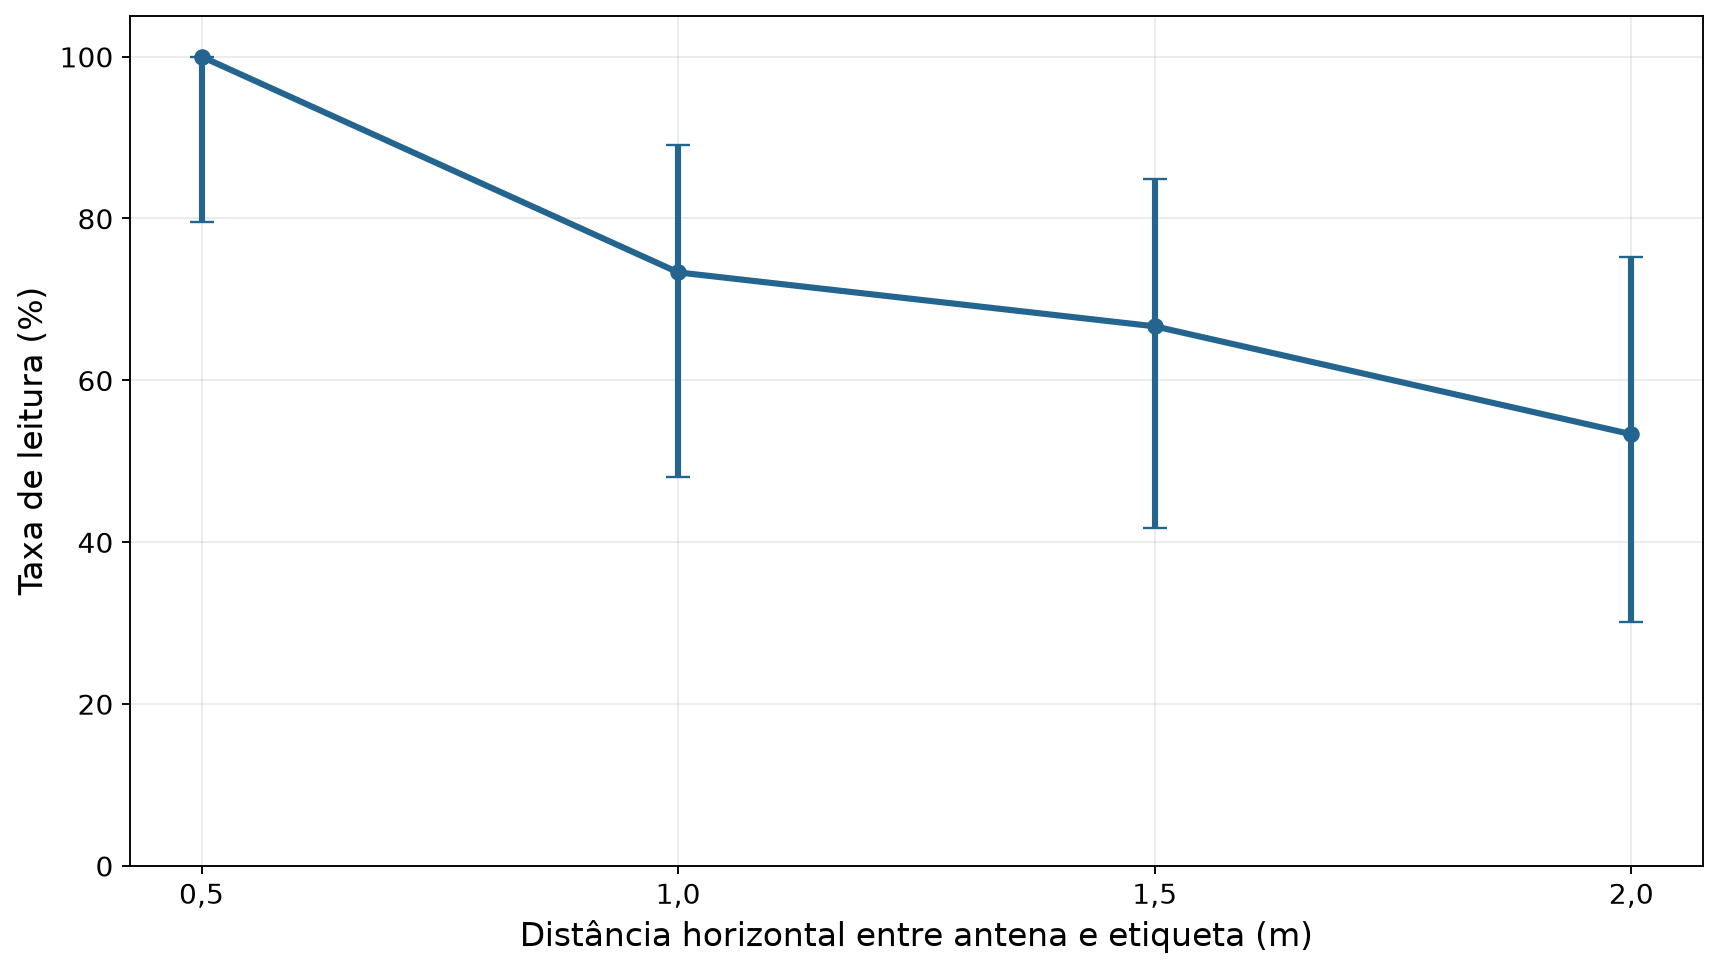
\includegraphics[width=0.82\textwidth]{./04-figuras/resultado_alcance_distancia}
    \fonte{Elaborado pelo autor a partir dos dados experimentais (2026).}
\end{figure}

\FloatBarrier

Adotando 90\% como limiar diagnóstico de repetibilidade por condição, apenas o ponto de 0,5~m atingiu o critério nesta campanha. Como a próxima distância ensaiada foi 1,0~m, os dados não permitem localizar com precisão o limite entre esses dois pontos. Esse limiar não constitui aceitação operacional para o inventário, pois detectar 90\% das tentativas ou dos bens ainda deixa omissões. Para uma passagem pela sala, o requisito adotado é identificar todos os EPCs esperados na mesma rodada.

Na \autoref{tab:resultado-alcance-distancia}, o tempo médio até a primeira leitura, calculado somente entre tentativas com detecção, cresce com a distância: $0{,}020 \pm 0{,}003$~s a 0,5~m, $0{,}206 \pm 0{,}338$~s a 1,0~m, $0{,}596 \pm 0{,}726$~s a 1,5~m e $0{,}773 \pm 0{,}846$~s a 2,0~m. A dispersão elevada nos três últimos pontos mostra que a média temporal deve ser interpretada com cautela; tentativas sem detecção não entram nesse cálculo e já são representadas pela taxa de sucesso. As médias de RSSI bruto também não variaram de forma monotônica com a distância. Como o RSSI não foi calibrado e o multipercurso integrou o cenário realista sem ser medido separadamente, esses valores descrevem apenas o comportamento relativo observado; eles não podem ser convertidos para potência em dBm nem utilizados para isolar causalmente os mecanismos de propagação. Além disso, TAG1, TAG2 e TAG3 permaneceram associadas, respectivamente, a papelão, madeira e plástico. Como os mesmos três conjuntos foram usados em todas as distâncias, a comparação agregada entre distâncias conserva a composição do painel, mas uma diferença individual não pode ser atribuída somente à etiqueta.

\section{Orientação}

A \autoref{tab:resultado-orientacao} mostra que o conjunto obteve 93,3\% de leitura em 0$^\circ$, 86,7\% em 45$^\circ$ e 66,7\% em 90$^\circ$, sempre a 1,5~m. Os intervalos de confiança de 95\% foram, respectivamente, de 70,2\% a 98,8\%, de 62,1\% a 96,3\% e de 41,7\% a 84,8\%. A tendência monotônica é compatível com a perda de acoplamento por desalinhamento entre polarizações lineares. Em um cenário institucional fechado, o multipercurso faz parte das condições normais de operação. Como os intervalos se sobrepõem e esse efeito não foi medido separadamente, os dados não permitem atribuir toda a diferença exclusivamente ao ângulo. Os três conjuntos formados por etiqueta e suporte aparecem em todos os ângulos, mas a associação fixa entre exemplar e suporte permanece como fator de confusão na análise individual.

\TabelaOrientacao

A \autoref{fig:resultado-orientacao} permite comparar visualmente a tendência entre os três ângulos, preservando a amplitude dos intervalos de confiança.

\begin{figure}[htbp]
    \centering
    \caption{Taxa experimental de leitura nas orientações testadas a 1,5~m; as barras de erro representam o IC 95\% de Wilson.}
    \label{fig:resultado-orientacao}
    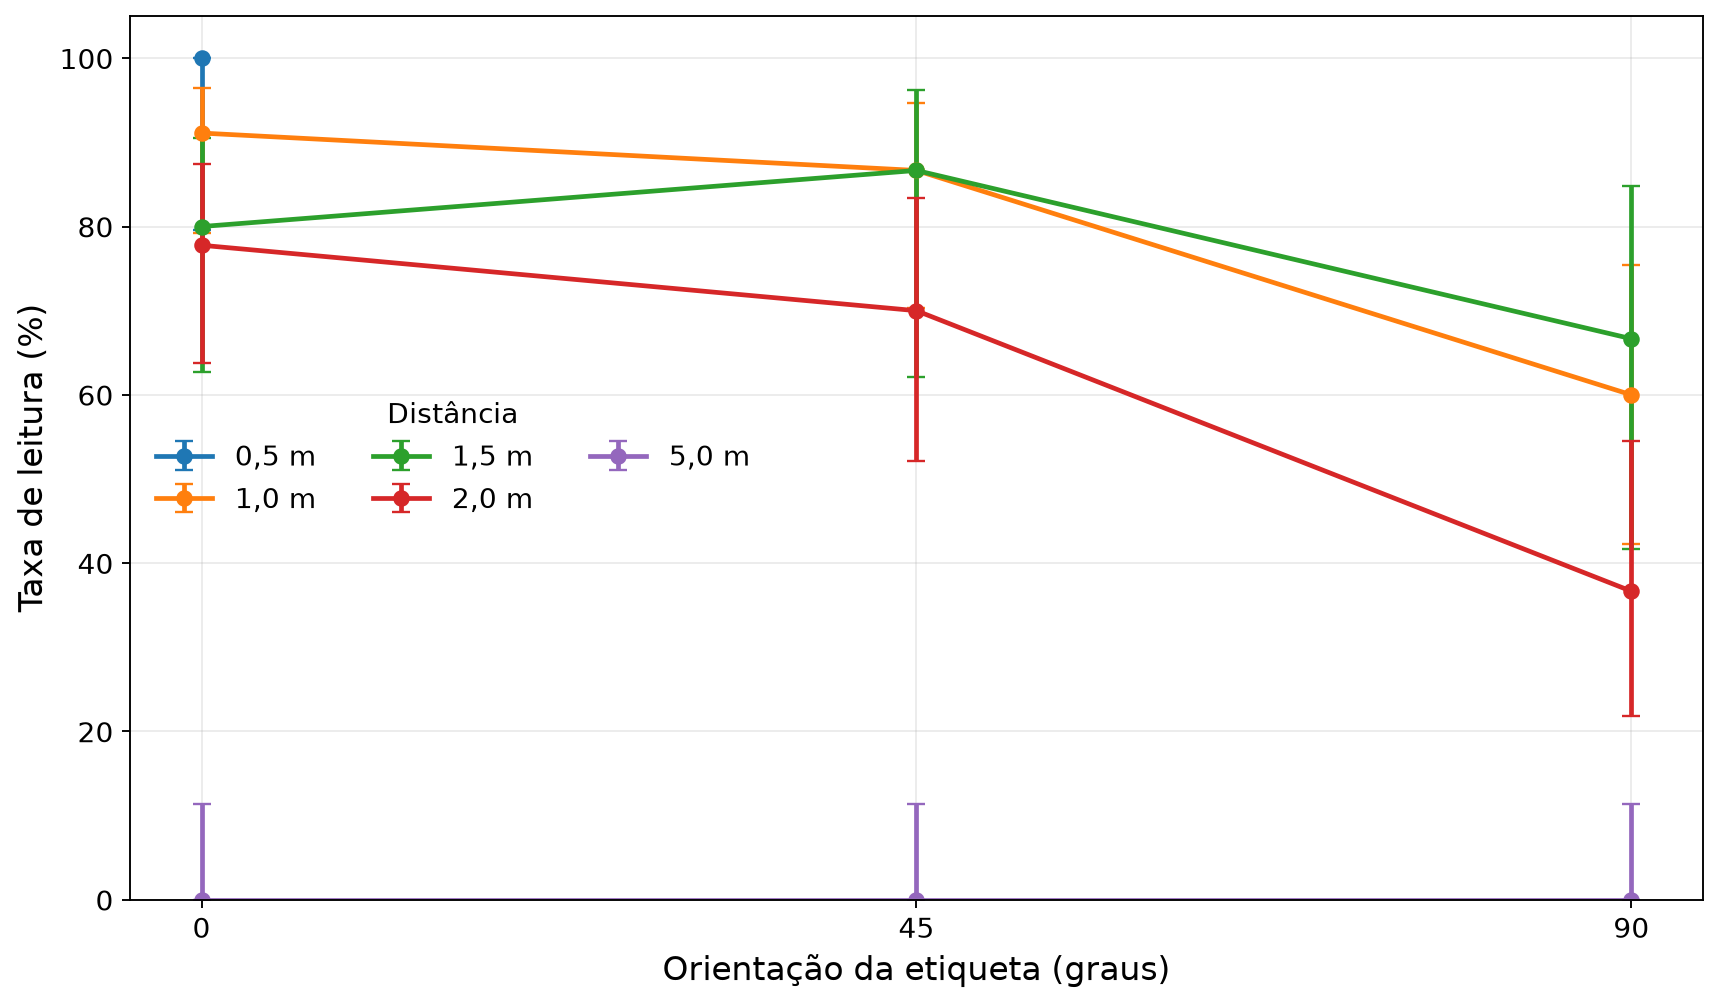
\includegraphics[width=0.70\textwidth]{./04-figuras/resultado_orientacao}
    \fonte{Elaborado pelo autor a partir dos dados experimentais (2026).}
\end{figure}

A análise complementar por conjunto formado por etiqueta e suporte é apresentada na \autoref{tab:resultado-por-tag}.

\TabelaPorEtiqueta

\FloatBarrier

A \autoref{tab:resultado-por-tag} apresenta uma verificação complementar por conjunto. No ensaio de distância, TAG1 com papelão, TAG2 com madeira e TAG3 com plástico obtiveram, respectivamente, 75,0\%, 85,0\% e 60,0\%; no ensaio de orientação, as taxas foram 86,7\%, 86,7\% e 73,3\%. Essa variação descreve os conjuntos efetivamente usados, mas não permite concluir que uma etiqueta, madeira ou plástico foi responsável pela diferença, pois exemplar e suporte não foram variados independentemente.

\section{Ensaio complementar com uma etiqueta isolada}

A \autoref{tab:resultado-ensaio-uma-tag} reúne o ensaio complementar com uma única etiqueta na zona de leitura. Em 1,0~m, as taxas foram 100,0\%, 86,7\% e 60,0\% para 0$^\circ$, 45$^\circ$ e 90$^\circ$. Em 2,0~m, os valores caíram para 90,0\%, 70,0\% e 36,7\%. Em 5,0~m, não houve detecção nas 30 tentativas de cada orientação. Os intervalos de Wilson permanecem apresentados porque, mesmo com 30 tentativas por combinação, as proporções não constituem valores exatos da população.

\TabelaEnsaioUmaTag

O bloco complementar evidencia uma interação prática entre distância e orientação: o alinhamento de 0$^\circ$ preservou desempenho elevado em 1,0 e 2,0~m, enquanto o desalinhamento reduziu a repetibilidade, e 5,0~m ficou fora do alcance útil nas condições observadas. Como essas falhas ocorreram com apenas uma etiqueta respondendo, colisões entre tags não são necessárias para explicar parte das omissões. O multipercurso, o limiar de energização da tag, a polarização, a aquisição serial e outras fontes de variabilidade ainda podem atuar. O ensaio não quantifica a contribuição de colisões no inventário; isso exigiria comparar, na mesma geometria e sob o mesmo protocolo, cada etiqueta isolada e as mesmas etiquetas presentes simultaneamente.

Os registros desse bloco foram preservados apenas como contagens consolidadas. Eles não contêm RSSI, tempos individuais, ordem das tentativas ou diagnósticos seriais suficientes para combinação com os demais ensaios. Por essa razão, a matriz complementa a interpretação de distância e orientação, mas não altera as estatísticas das tabelas anteriores.

\FloatBarrier

\section{Material de fixação}

Na \autoref{tab:resultado-material}, papelão e metal com espaçador plástico de 10~mm apresentaram 100,0\% de leitura, enquanto o metal direto resultou em 0,0\%. Como houve apenas cinco tentativas e um único exemplar de tag por condição, os intervalos de 95\% ainda são amplos: de 56,6\% a 100,0\% nos dois casos de sucesso integral e de 0,0\% a 43,4\% no metal direto.

\TabelaMaterial

A \autoref{fig:resultado-material} destaca o contraste entre o contato metálico direto e as duas condições nas quais houve detecção.

\begin{figure}[htbp]
    \centering
    \caption{Taxa experimental de leitura para os materiais de fixação testados; as barras de erro representam o IC 95\% de Wilson.}
    \label{fig:resultado-material}
    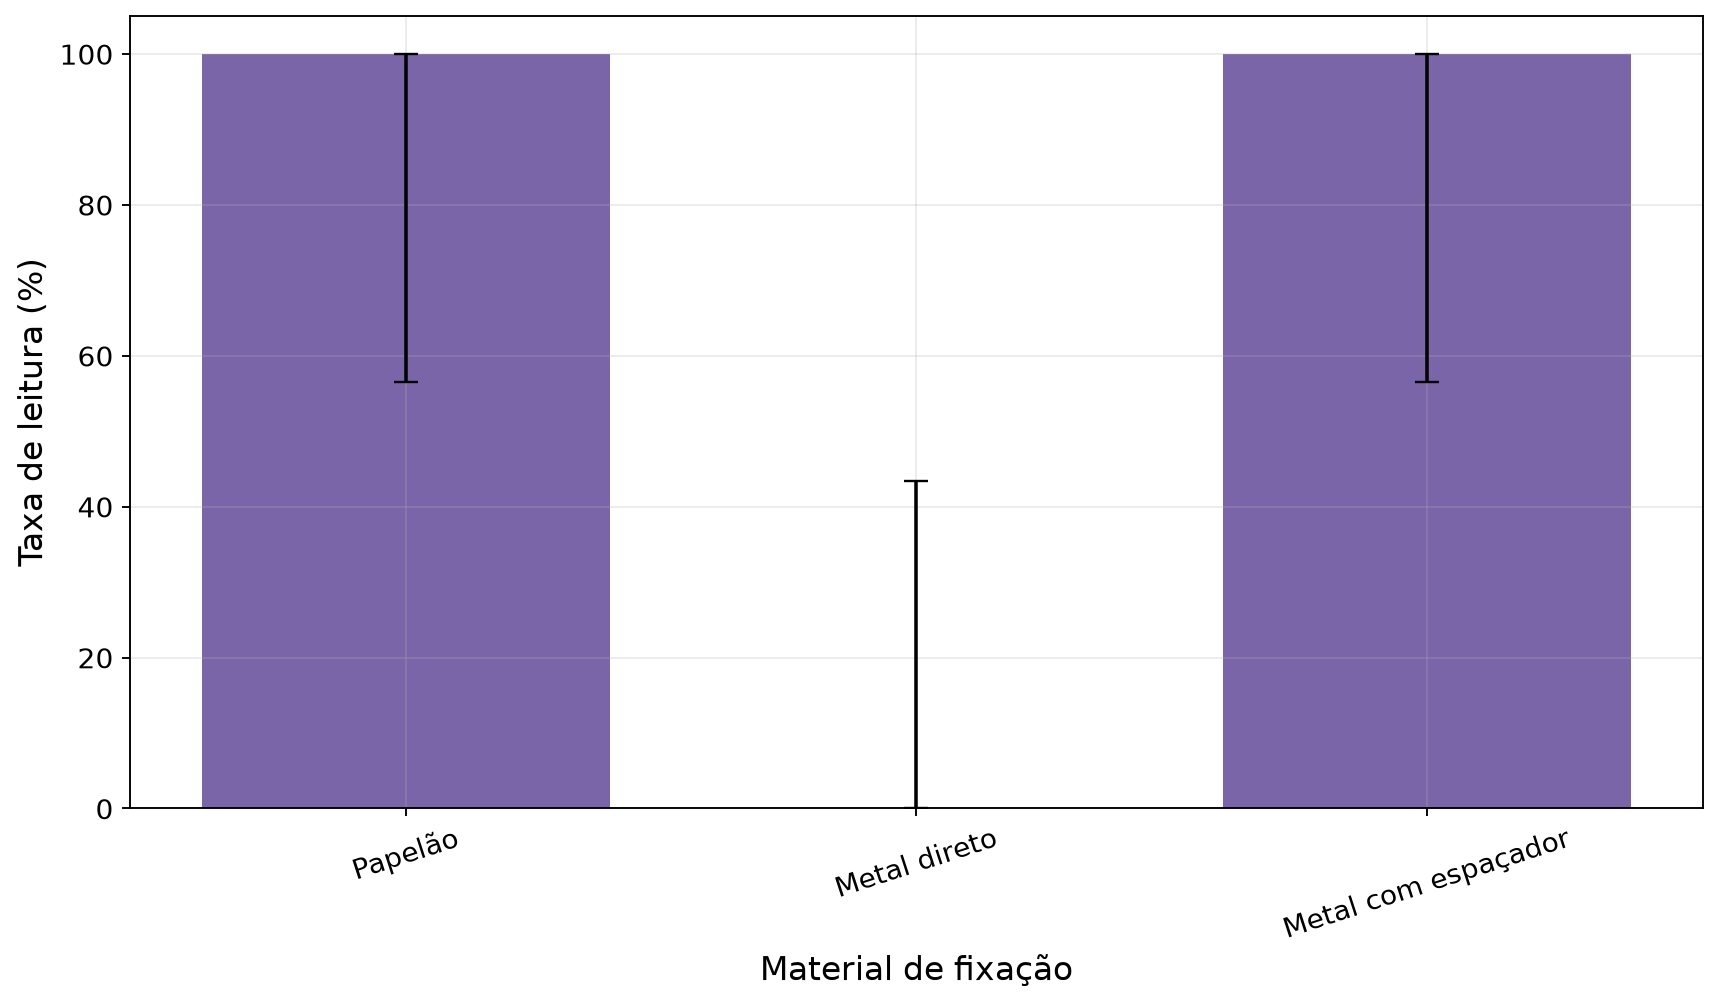
\includegraphics[width=0.82\textwidth]{./04-figuras/resultado_material}
    \fonte{Elaborado pelo autor a partir dos dados experimentais (2026).}
\end{figure}

\FloatBarrier

O espaçador de 10~mm recuperou a leitura nas cinco tentativas realizadas, fornecendo evidência favorável à separação física nessa montagem. O resultado não permite definir 10~mm como espessura ótima nem substituir a validação com etiquetas próprias para metal. Para a prática patrimonial, ele indica que bens metálicos exigem etiqueta adequada ou suporte auxiliar previamente testado.

\section{Inventário em sala}

O inventário em sala apresentou cobertura de 80\% nas rodadas 1 a 4 e de 60\% na rodada 5, com média de 76,0\%, desvio-padrão de 8,9 pontos percentuais e IC 95\% da média de 64,9\% a 87,1\%. Nenhuma das cinco rodadas foi completa. Portanto, a taxa observada de inventários completos foi de 0,0\%, com IC 95\% de Wilson de 0,0\% a 43,4\%. O intervalo da cobertura média informa quantas etiquetas foram encontradas, em média, e não a chance de concluir a conferência. A taxa de rodadas completas é a métrica diretamente relacionada ao requisito de identificar todos os bens em uma passagem. As tags foram avaliadas ao longo de um percurso curto padronizado em laboratório fechado de aproximadamente 50~m$^2$, configuração compatível com uma operação cotidiana de inventário institucional. Como dimensões lineares, coordenadas individuais e trajeto exato não foram registrados, não é possível reproduzir integralmente a geometria, mas essa ausência não descaracteriza a avaliação do desempenho agregado no cenário de uso. A \autoref{tab:resultado-inventario-rodadas} detalha cada rodada e a \autoref{tab:resultado-inventario} reúne os indicadores consolidados.

\TabelaInventarioRodadas
\TabelaInventarioResumo

A \autoref{fig:resultado-inventario} mostra a estabilidade das quatro primeiras rodadas e a redução observada na quinta.

\begin{figure}[htbp]
    \centering
    \caption{Cobertura por rodada no inventário experimental em sala.}
    \label{fig:resultado-inventario}
    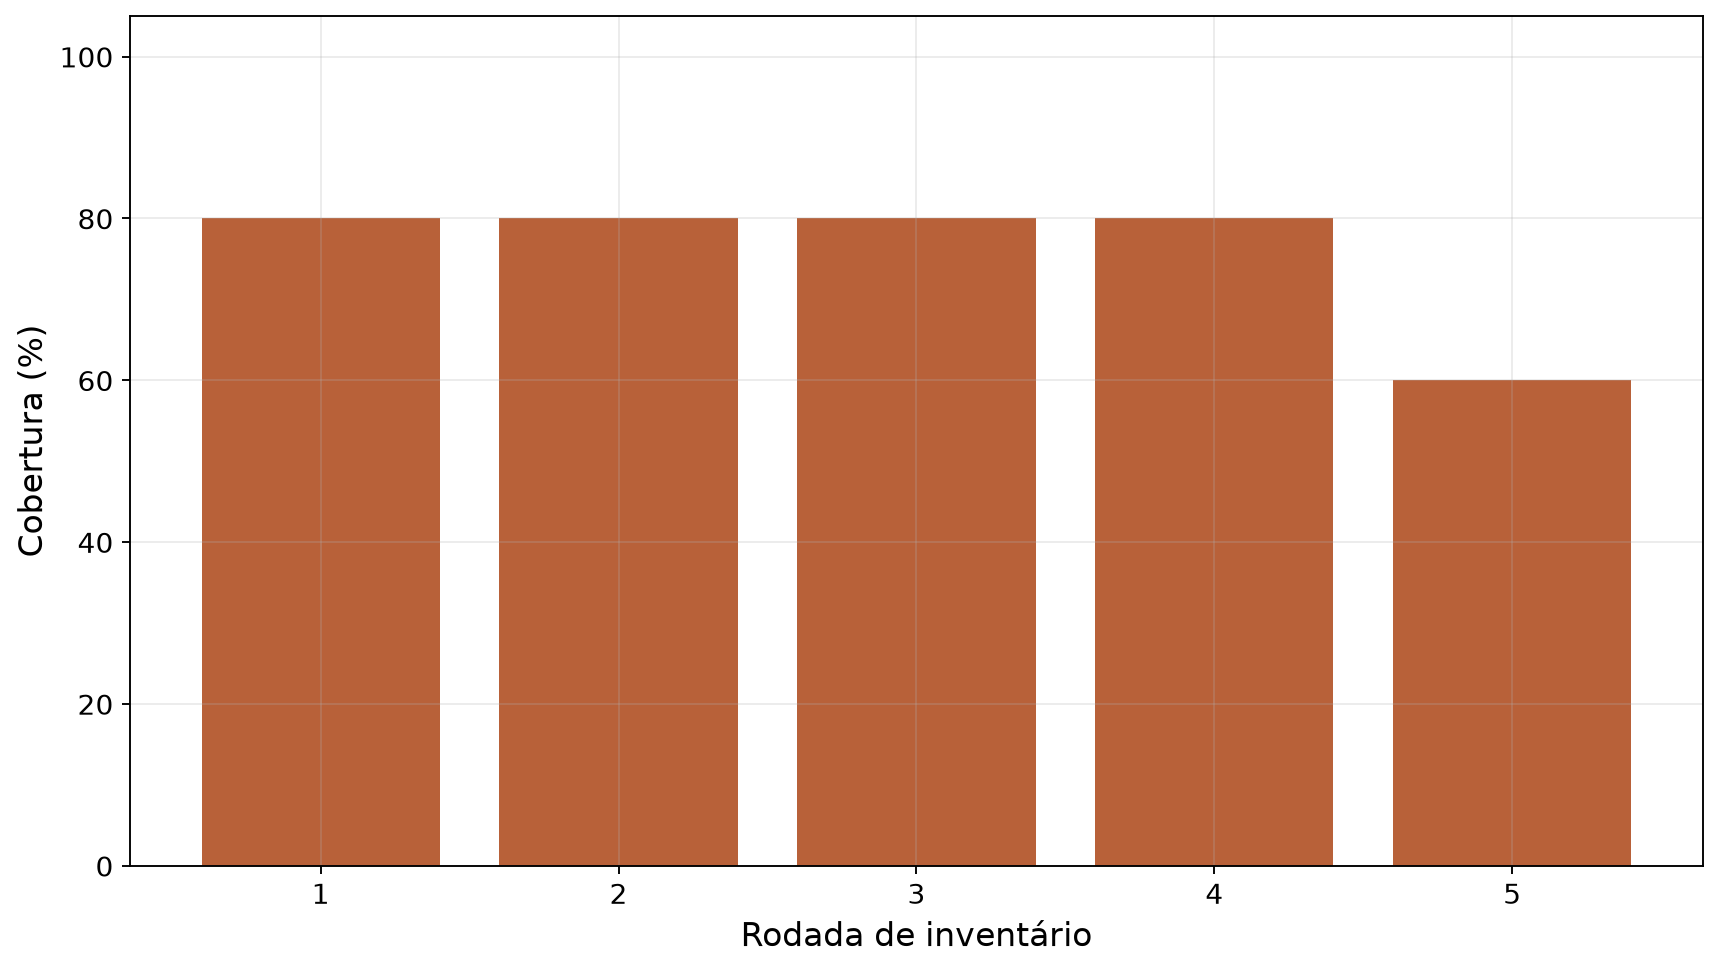
\includegraphics[width=0.82\textwidth]{./04-figuras/resultado_inventario}
    \fonte{Elaborado pelo autor a partir dos dados experimentais (2026).}
\end{figure}

\FloatBarrier

A ausência de rodadas completas mostra que, em ambiente comum e com apenas uma antena, a cobertura média não basta para garantir inventário completo. O IC da taxa de rodadas completas é amplo devido às cinco rodadas e não demonstra que a probabilidade real seja exatamente zero. Ainda assim, nenhuma execução satisfez o requisito, de modo que os dados não sustentam o uso da configuração atual como referência operacional. Foram registrados 73 quadros válidos: 19 correspondem às detecções distintas somadas entre as rodadas e 54 foram repetições de EPC já visto na mesma janela. Não houve leitura externa nas cinco rodadas oficiais. O firmware deduplicou esses quadros antes de calcular a cobertura, conforme definido na metodologia. A presença aproximada de cinco pessoas e quatro objetos metálicos próximos caracteriza uma condição usual de laboratório e aumenta a representatividade prática do ensaio. Como esses elementos não foram variados independentemente, os resultados descrevem o desempenho do conjunto no cenário completo, e não o efeito isolado de cada componente ambiental.

As cinco etiquetas formavam a etapa inicial de uma progressão planejada até aproximadamente 50 unidades. Como a cobertura integral não ocorreu sequer nessa etapa, aumentar a população não permitiria corrigir a limitação física já observada. O escalonamento foi interrompido para priorizar a revisão de antena, etiquetas, geometria e configuração do leitor. Essa decisão não estabelece que cinco seja a capacidade máxima do YPD-R200; a capacidade de inventário do protocolo não foi medida, pois o critério mínimo de desempenho da montagem falhou antes do teste de escala.

\section{Integridade da aquisição}

Após as medições, verificou-se que a alternância entre a fonte externa de 5~V/1~A e a alimentação pela conexão USB do Arduino não produziu alteração relevante nos resultados obtidos.

Os registros diagnósticos coletados permitem avaliar a aquisição sem atribuir automaticamente toda falha à interface de RF. Nas 693 consultas dos ensaios principais de distância, orientação e material, ocorreram 21 quadros inválidos (3,0\%), 9 \textit{timeouts} (1,3\%) e nenhum erro de comando. No inventário, foram 251 consultas, 5 quadros inválidos (2,0\%), 2 \textit{timeouts} (0,8\%) e nenhum estouro da tabela de EPCs. O ensaio complementar de uma etiqueta não integra essas contagens, pois seus registros foram preservados apenas de forma agregada. Esses percentuais são diagnósticos do programa, e não uma taxa de erro de enquadramento da UART: sem analisador lógico, não é possível distinguir completamente corrupção em \texttt{SoftwareSerial}, resposta malformada do módulo e efeitos do enlace entre leitor e tag.

\section{Síntese da discussão}

Os resultados sustentam as três tendências principais da hipótese: a repetibilidade caiu com a distância, o contato direto com metal impediu a detecção da etiqueta convencional e a taxa diminuiu com o aumento do desalinhamento angular. O ensaio de etiqueta isolada mostra que existem falhas sem disputa simultânea entre tags, de modo que colisão não pode ser tratada como explicação exclusiva para o inventário incompleto. A campanha não separou estatisticamente polarização, multipercurso, suporte, exemplar, serial e anticolisão. Os dados também mostram que o inventário com cinco tags não fechou nenhuma janela, reforçando a necessidade de acumular EPCs únicos, registrar omissões e melhorar a configuração física antes de aumentar a escala.

Em termos de escolha de antena, a APCA8090 linear permitiu estabelecer uma linha de base experimental de baixo custo, mas a configuração não atingiu o requisito operacional. Para tratar diretamente a sensibilidade à orientação, a comparação futura prioritária é com polarização circular ou diversidade de polarização. Uma antena omnidirecional constitui hipótese separada para ampliar a cobertura azimutal e reduzir o esforço de apontamento; ela não corrige por si só o desalinhamento de polarização e pode elevar leituras externas e multipercurso. Bens metálicos também exigem comparar o espaçador com etiquetas próprias para metal.

\section{Requisitos derivados para evolução do protótipo}

Os requisitos da \autoref{tab:requisitos-evolucao} são derivados da campanha. A coluna relativa ao ponto fixo apresenta especificações para trabalho futuro, e não resultados experimentais, pois não houve ensaio de passagem em portal ou zona fixa.

\begin{table}[H]
    \centering
    \caption{Requisitos derivados dos resultados para os cenários portátil e fixo.}
    \label{tab:requisitos-evolucao}
    \footnotesize
    \begin{tabularx}{\textwidth}{p{3.0cm}X X}
        \toprule
        \textbf{Aspecto} & \textbf{Leitor portátil} & \textbf{Ponto fixo} \\
        \midrule
        Zona de leitura & Procedimento deve aproximar a antena das tags e exigir cobertura integral por passagem; 90\% por condição é insuficiente para aceitação. & Cobertura deve ser confinada para reduzir leituras de áreas adjacentes e validada na geometria real da passagem. \\
        Antena e etiquetas & Comparar a APCA8090 com polarização circular ou diversa, avaliar cobertura azimutal e usar tags próprias para metal quando necessário. & Preferir cobertura controlada; inferência de direção exige duas zonas, duas antenas ou sensor auxiliar. \\
        Eletrônica & Usar UART de hardware, confirmar adequação de nível lógico e dimensionar alimentação para o pico do leitor. & Registrar canal/região, potência efetiva e estabilidade em operação prolongada. \\
        Software & Persistir EPC, instante, ambiente e estado da janela; deduplicar antes de calcular cobertura. & Correlacionar eventos por zona e tempo, sem classificar presença isolada como entrada ou saída. \\
        Validação & Após melhorar a configuração, exigir rodadas completas com cinco tags e somente então ampliar gradualmente a população até aproximadamente 50, em mais sessões e ambientes. & Medir leituras externas, omissões e falsos eventos em percursos nos dois sentidos. \\
        \bottomrule
    \end{tabularx}
    \fonte{Elaborado pelo autor a partir dos resultados da campanha (2026).}
\end{table}

    %
% Documento: Conclusão
%

\chapter{Considerações finais}
\label{cap:conclusao}

Este trabalho substituiu a concepção inicial baseada em NFC por uma arquitetura RFID UHF mais compatível com a leitura de múltiplos bens durante uma varredura. Foram especificados o YPD-R200, a antena APCA8090, a etiqueta AD-239 M730 e o Arduino, e o firmware foi adaptado para a abstração \texttt{Stream}, comando nominal de potência e EPCs de tamanho variável.

A validação física planejada não foi realizada. A decisão de empregar simulação decorreu do tempo insuficiente para aquisição, montagem, ensaios piloto e repetições controladas e do custo de múltiplas antenas, etiquetas, instrumentação, estruturas de posicionamento e acesso a um ambiente controlado. Consequentemente, todas as taxas, RSSIs, rotas, passagens e janelas apresentadas são dados sintéticos. Eles não comprovam o desempenho do protótipo real.

No modelo, a taxa média simulada de leitura foi de 96,9\% a 0,5~m, 95,1\% a 1,0~m, 93,1\% a 1,5~m e 90,0\% a 2,0~m, caindo para 77,8\% a 2,5~m e 48,0\% a 3,0~m. Mesmo a 1,5~m, somente 10 das 15 configurações tag--altura atingiram individualmente o critério interno de 90\%, mostrando que a média da simulação pode ocultar condições desfavoráveis.

As taxas geradas para orientação foram de 89,1\%, 53,8\% e 10,0\% a $0^\circ$, $45^\circ$ e $90^\circ$. Essa queda foi produzida pela penalidade angular do modelo e não constitui medição da APCA8090. Para materiais, a simulação gerou 3,3\% sobre metal direto e 30,0\% com espaçador de 10~mm, em contraste com 80,0\% a 100,0\% nas superfícies não metálicas representadas.

No inventário virtual, a cobertura média foi de 91,0\%, com omissão de 9,0\%, mas somente três das dez janelas foram completas. Também foram geradas 298 duplicatas e duas leituras externas. Esses resultados exercitam as métricas e reforçam conceitualmente a necessidade de contar EPCs únicos; não demonstram confiabilidade operacional nem comprovam que o firmware atual realize essa consolidação.

A pergunta de pesquisa foi respondida somente no domínio do modelo: sob suas premissas, distância, orientação e material alteram fortemente as taxas projetadas, e a média de cobertura não basta para definir um inventário confiável. A hipótese apresentou coerência interna, mas não foi validada empiricamente. O trabalho deve ser entendido como arquitetura de protótipo acompanhada de análise exploratória e protocolo para futura experimentação.

Quanto à antena, uma alternativa omnidirecional pode ser mais adequada à varredura portátil quando a prioridade é ampliar a cobertura azimutal e reduzir o apontamento pelo operador. A simulação atual, entretanto, não comparou antenas e não permite declarar sua superioridade. Para reduzir a dependência da orientação das tags, a comparação mais direta continua sendo uma antena circular ou com diversidade de polarização. A escolha futura deve avaliar conjuntamente padrão de irradiação, polarização, ganho, leituras externas e ergonomia; para um portal fixo, o controle espacial de uma antena direcional pode ser preferível.

\section{Limitações e continuidade}

A principal limitação é o caráter integralmente sintético da base. O modelo é fenomenológico, não eletromagnético, e não foi calibrado com medições. Ele simplifica multipercurso, resposta de materiais, variação entre etiquetas, geometria, protocolo Gen2 e falhas da interface serial. Os percentuais dependem das regras adotadas e não devem ser generalizados para o YPD-R200, a APCA8090 ou outras instalações.

Embora a planilha registre sementes e preserve todas as 6.330 tentativas controladas e os 400 registros de inventário, o código original do gerador, seus coeficientes e a função de conversão para probabilidade não estão no repositório. Assim, os agregados são auditáveis a partir da base, mas a geração não é integralmente reproduzível do zero. Uma evolução prioritária é versionar o gerador completo ou reconstruir um modelo documentado e calibrá-lo com uma coleta piloto.

O firmware também permanece incompleto para inventário real: armazena apenas o último EPC, não mantém uma tabela de EPCs únicos por janela, não grava RSSI bruto, timestamp e condição experimental e não confirma região, canal, FHSS ou potência aplicada. Esses requisitos devem ser implementados antes de qualquer comparação entre dados físicos e simulados.

Como continuidade, recomenda-se realizar inicialmente uma campanha reduzida e financeiramente viável, preservando log serial integral, fotografias, geometria, versão do firmware e configuração do leitor. Em seguida, deve-se comparar a antena linear de referência com uma alternativa circular ou de diversidade de polarização e uma alternativa omnidirecional, usando as mesmas tags, cabos, potência e ambiente. Para bens metálicos, devem ser incluídas etiquetas próprias para metal. Somente após essa calibração será possível revisar o modelo, quantificar sua aderência e concluir sobre o desempenho operacional do protótipo.


    \postextual
    %
% Documento: Referências Bibliográficas
%

\bibliography{./bibliografia}  

\end{document}
